\chapter{The system and the excitation signal}
\section{Introduction}
The goal of this lab is to gain experience 
with the tools for identifying LTI systems described 
during the lectures. This will be applied to measurements on a real dynamic system. 
The system under consideration is the so-called \textit{Silverbox} system,
this is an electronic circuit which emulates a mass-spring damper system, with a nonlinear spring.  The system has a single input and a single output. The nonlinear spring in the feedback path follows the relation:

\begin{equation}
    y(t) = u(t)^3
\end{equation}

where $u(t)$ is the displacement and $y(t)$ is the restoring force. The system is excited with a designed excitation signal and the input and output signals are measured. The measurements are then used to estimate the system's frequency response function (FRF) using both non-parametric and parametric methods. Finally, a model order selection is performed to choose the best model for the system.

\section{Excitation signal}
The first step in the identification procedure is to design an appropriate excitation signal. 
The signal should be designed such that it excites the system in the frequency band of interest, and to design it such that it is possible to estimate nonlinear distortions. 

%After some experimatation, it could be seen that the dynamics of the system are mainly concentrated in the frequency band from 0 to 70 Hz. Therefore, the sampling frequency fs was chosen to be 7kHz. 

In the lectures we have seen two methods to design excitation signals that are suitable for nonlinear system identification:
\begin{enumerate}
    \item Robust method
    \item Fast method
\end{enumerate}

\subsection{Fast method} \label{sec:fast_method}

In the fast method, we design a multisine signal that excites only odd frequencies, leaving even frequencies unexcited. This allows us to estimate the nonlinear distortions by looking at the output at the unexcited frequencies. Not only do we only excite odd frequencies, we also leave some odd frequencies unexcited.
The multisine signal is defined in the frequency domain as:

\begin{equation}
    U(\omega_k) = \begin{cases}
    A_k e^{j \phi_k} & \omega_k = k \omega_0, k \in \mathcal{N} \\
    0 & \text{otherwise}
\end{cases}
\end{equation}

where $\mathcal{N}$ is a set of odd numbers that starts at the lowest frequency of interest and ends at the highest frequency of interest and where for a set of 4 consecutive odd numbers one is removed. $A_k$ is the amplitude of the k-th frequency component. They are all equal and chosen such that the rms value of the signal is equal to 0.1V. $\omega_0$ is the bin width, and $\phi_k$ is a random phase uniformly distributed between 0 and $2\pi$.


To design the multisine signal, you need to choose the sampling frequency $f_s$ and the number of samples $N$:

\begin{itemize}
    \item The sampling frequency should be chosen such that it is at least twice the highest frequency of interest, according to the Nyquist theorem. But in practice the sampling frequency is often chosen higher to account for non-idealities.
    \item The number of samples should be chosen such that the frequency resolution is sufficient to capture the dynamics of the system. The frequency resolution is given by $\Delta f = \frac{f_s}{N}$. A higher number of samples gives a better frequency resolution, but also increases the measurement time.
\end{itemize}


After some testing we choose a sampling frequency of $f_s = 4$ kHz and $N = 5000$ samples. This gives a frequency resolution of approximately $0.8 Hz$. The highest frequency of interest is around $1200 Hz$, which is well below the Nyquist frequency of $2000 Hz$.

\begin{figure}[H]
    \centering
    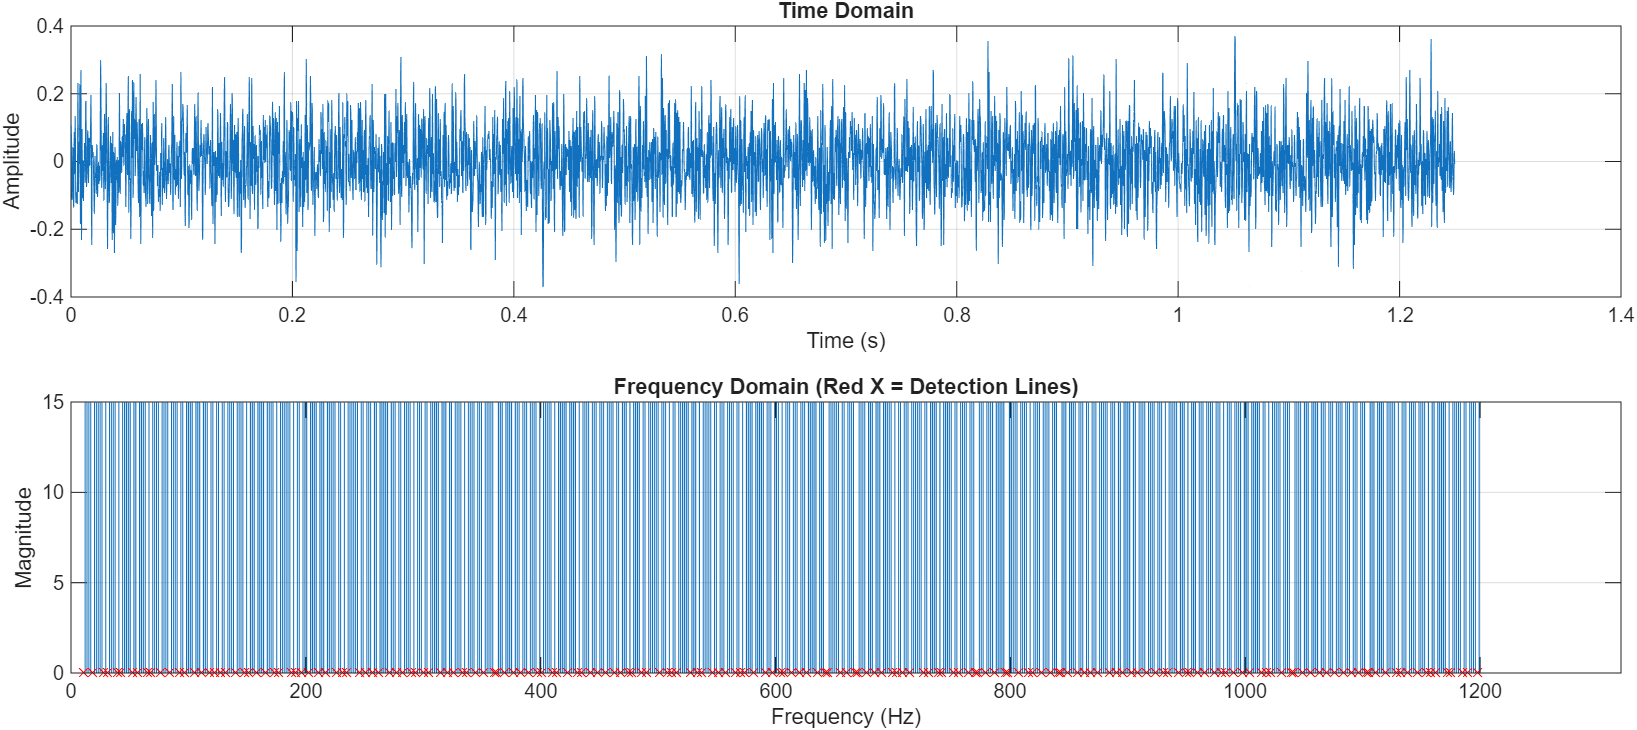
\includegraphics[width=0.7\textwidth]{pic/1_Fast_Method_Input_Signal.png}
    \caption{Excitation signal designed for the fast method in time and frequency domain}
    \label{fig:fast_multisine_time}
\end{figure}


\subsection{Robust method}

In the robust method, we design a multisine signal that excites all frequencies in the frequency band of interest. This allows us to estimate the nonlinear distortions by looking at the output at all frequencies. However, to be able to distinguish between nonlinear distortions and noise, we need to repeat the measurement multiple times with different random phase realizations.
The multisine signal is defined in the frequency domain in the same way as for the fast method, but now $\mathcal{N}$ contains not only 3/4 of the odd frequencies in the frequency band of interest but all frequencies in the frequency band of interest.



\begin{figure}[H]
    \centering
    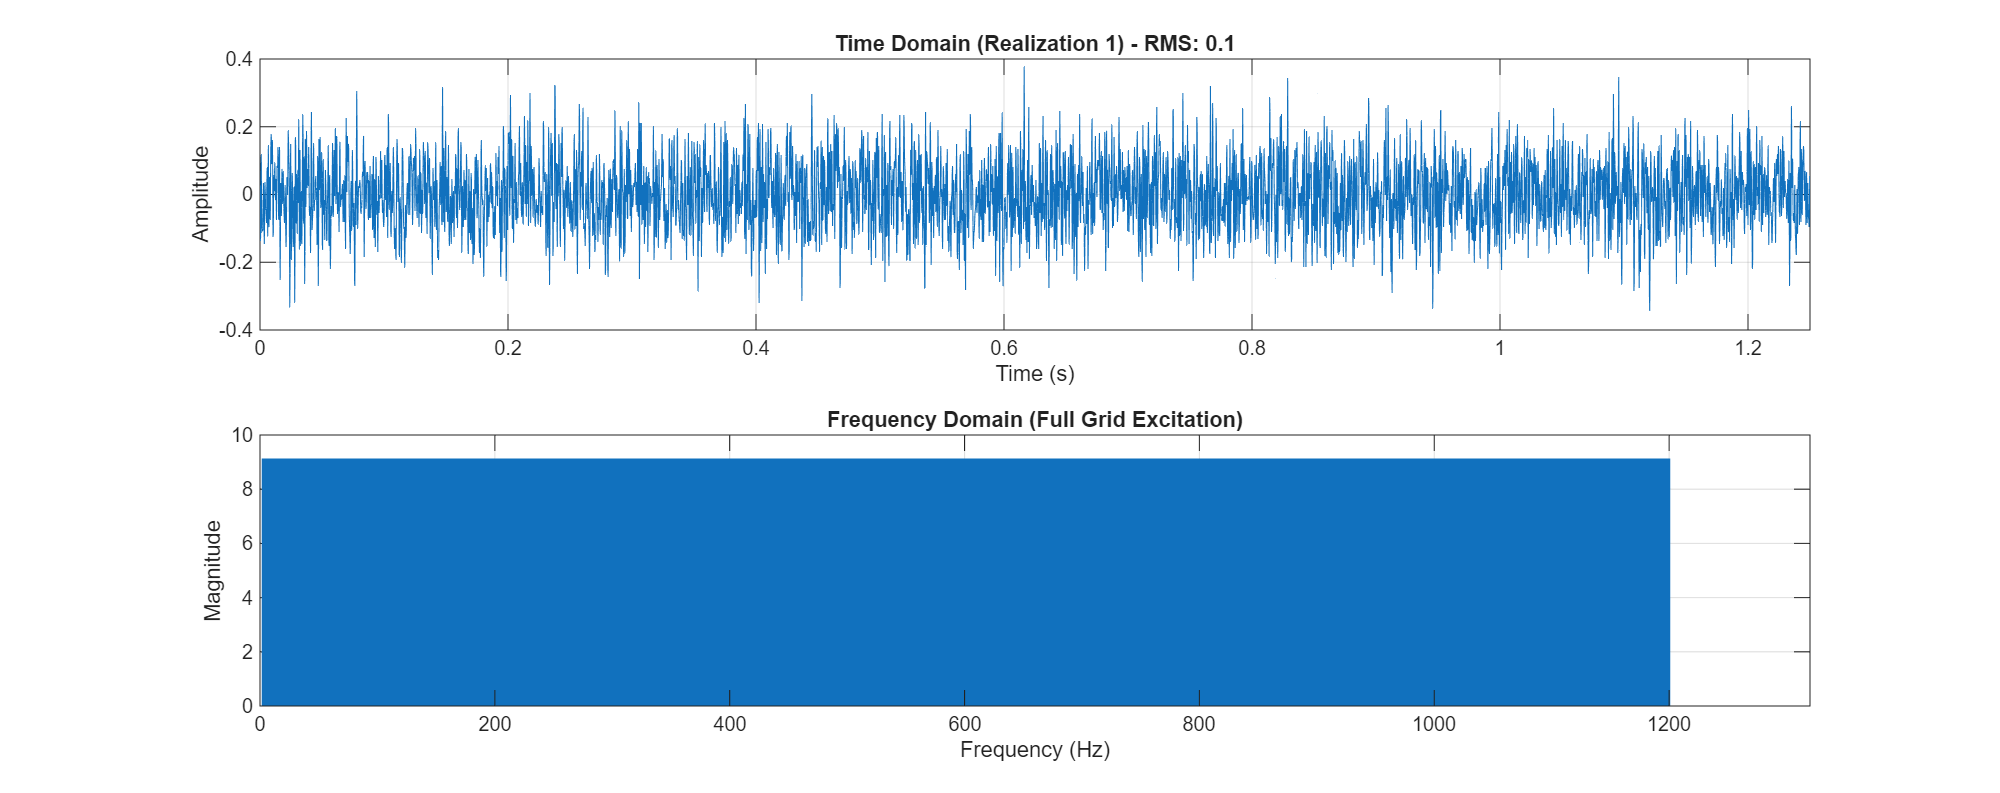
\includegraphics[width=0.7\textwidth]{pic/1_Robust_Method_Input_Signal.png}
    \caption{Excitation signal designed for the robust method in time and frequency domain}
    \label{fig:robust_multisine_time}
\end{figure}



\chapter{Non-Parametric Estimate of the System}

After exciting the system with the designed excitation signals, we can now estimate the system's frequency response function (FRF) using non-parametric methods.

\section{Non-parametric estimate}

In this section, we will estimate the FRF using the non-parametric method. The non-parametric method is based on the Fourier transform of the input and output signals at the excited frequencies only. 

\subsection{Fast method}

In the fast method, we can estimate the FRF using multiple periods of one realization. The FRF is estimated at the excited frequencies only, the set $\mathcal{N}$ defined in Section~\ref{sec:fast_method}. The even nonlinear distortions can be estimated by looking at the output at the even frequencies. The odd nonlinear distortions can be estimated by looking at the output at the unexcited odd frequencies. The noise level can be estimated by looking at the output at the added frequency bins due to the use of multiple periods.

\begin{figure}[H]
    \centering
    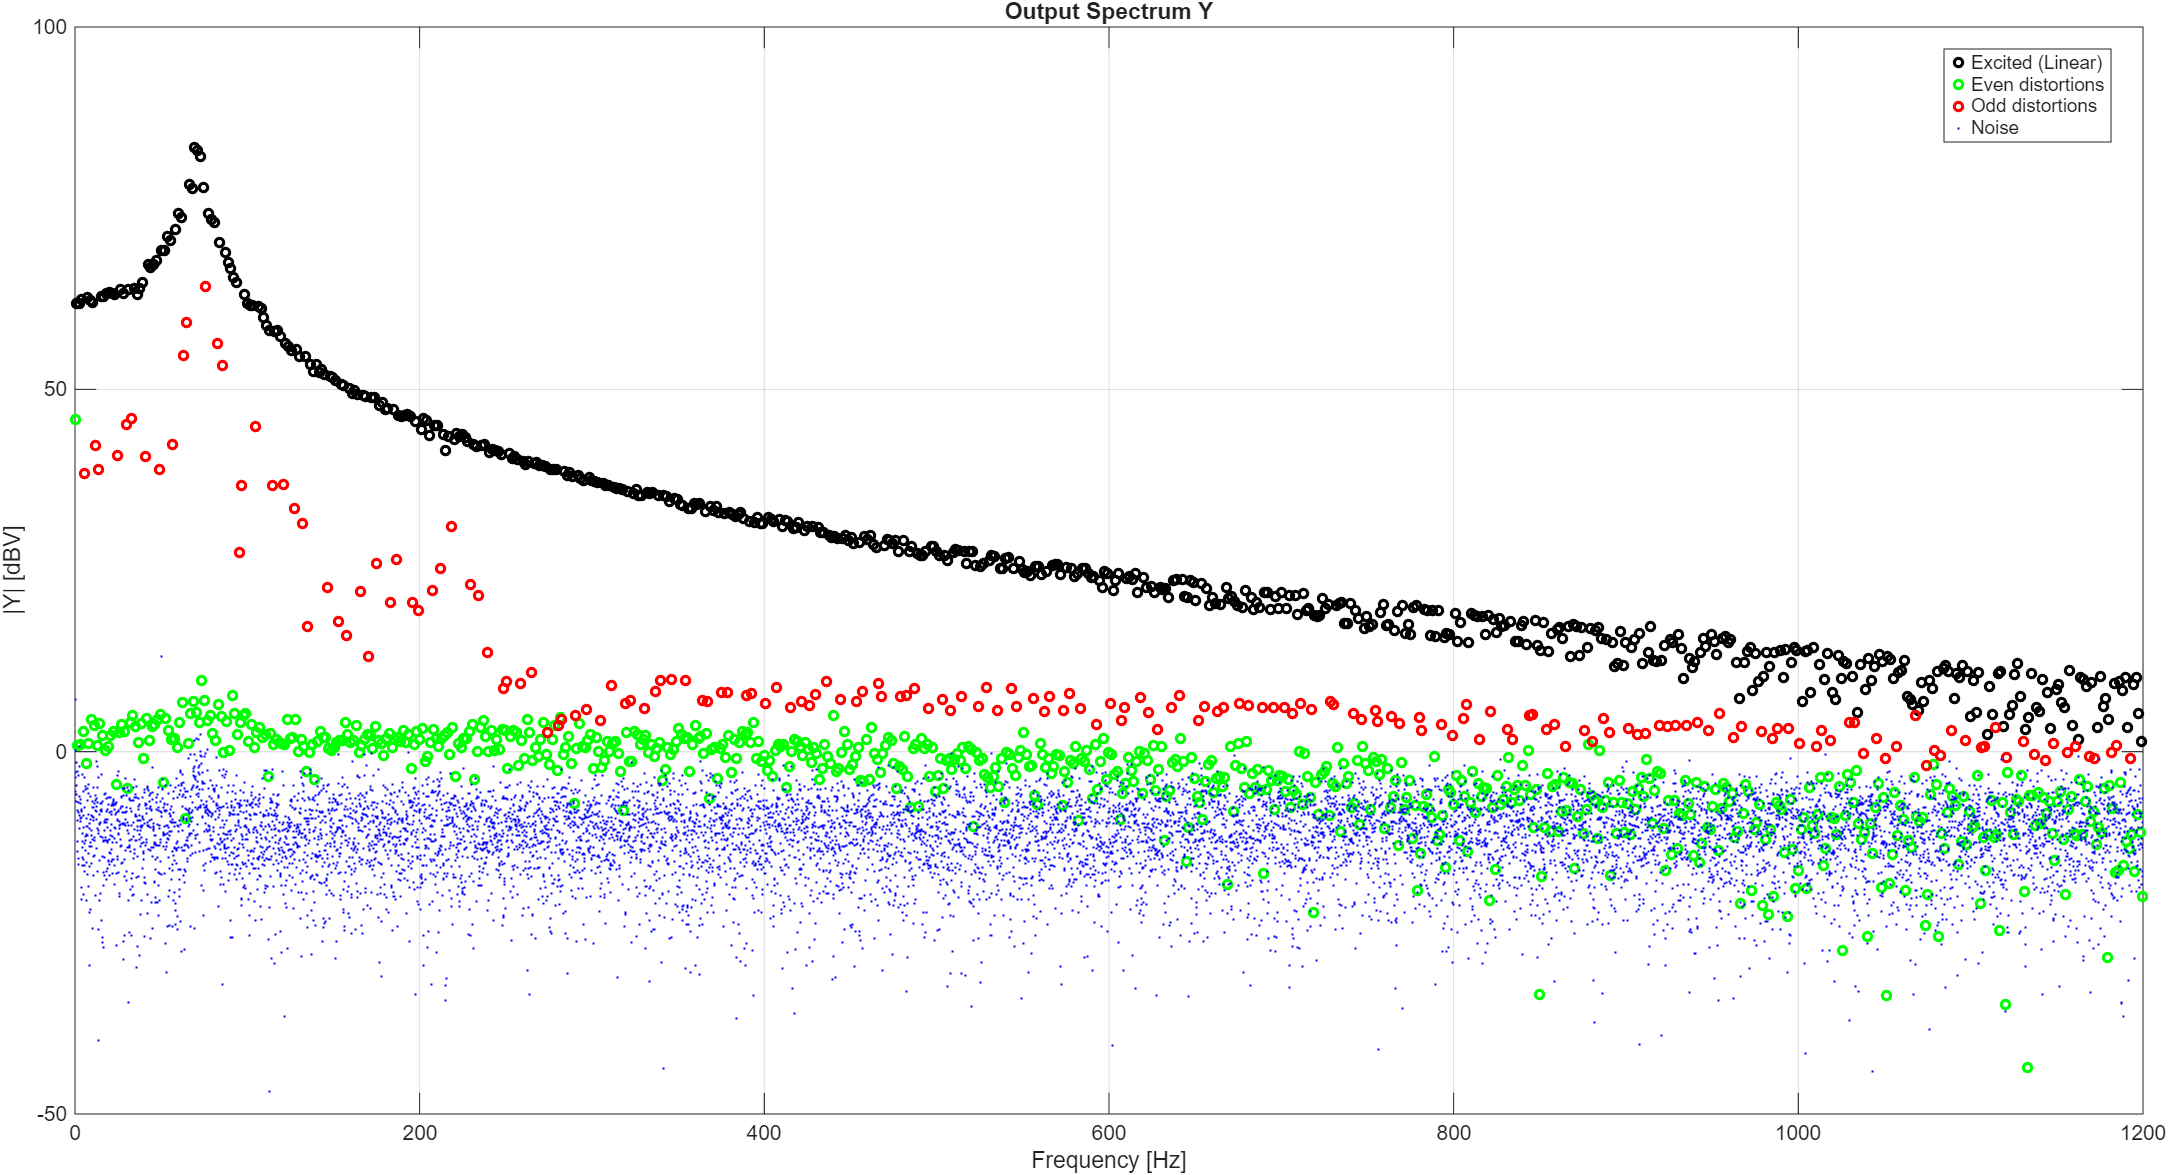
\includegraphics[width=1\textwidth]{pic/2_Fast_Method_Result.png}
    \caption{Output spectrum Y using the fast method}
    \label{fig:fast_FRF}
\end{figure}

As shown in Figure~\ref{fig:fast_FRF}, the output spectrum contains contributions from the linear system response, even nonlinear distortions, odd nonlinear distortions, and noise. 

At the excited frequencies (black), we see the linear response and the odd nonlinear distortions of the system. At the even frequencies (green), we see the even nonlinear distortions, which are significantly lower than the linear response. At the unexcited odd frequencies (red), we see the odd nonlinear distortions, which are higher than the even nonlinear distortions but still lower than the linear + odd response. Finally, at the added frequency bins (blue), we see the noise level, which is the lowest among all contributions.

As expected, the odd nonlinear distortions are predominant due to the cubic nonlinearity of the system. The even nonlinear distortions are significantly lower.



\begin{figure}[H]
    \centering
    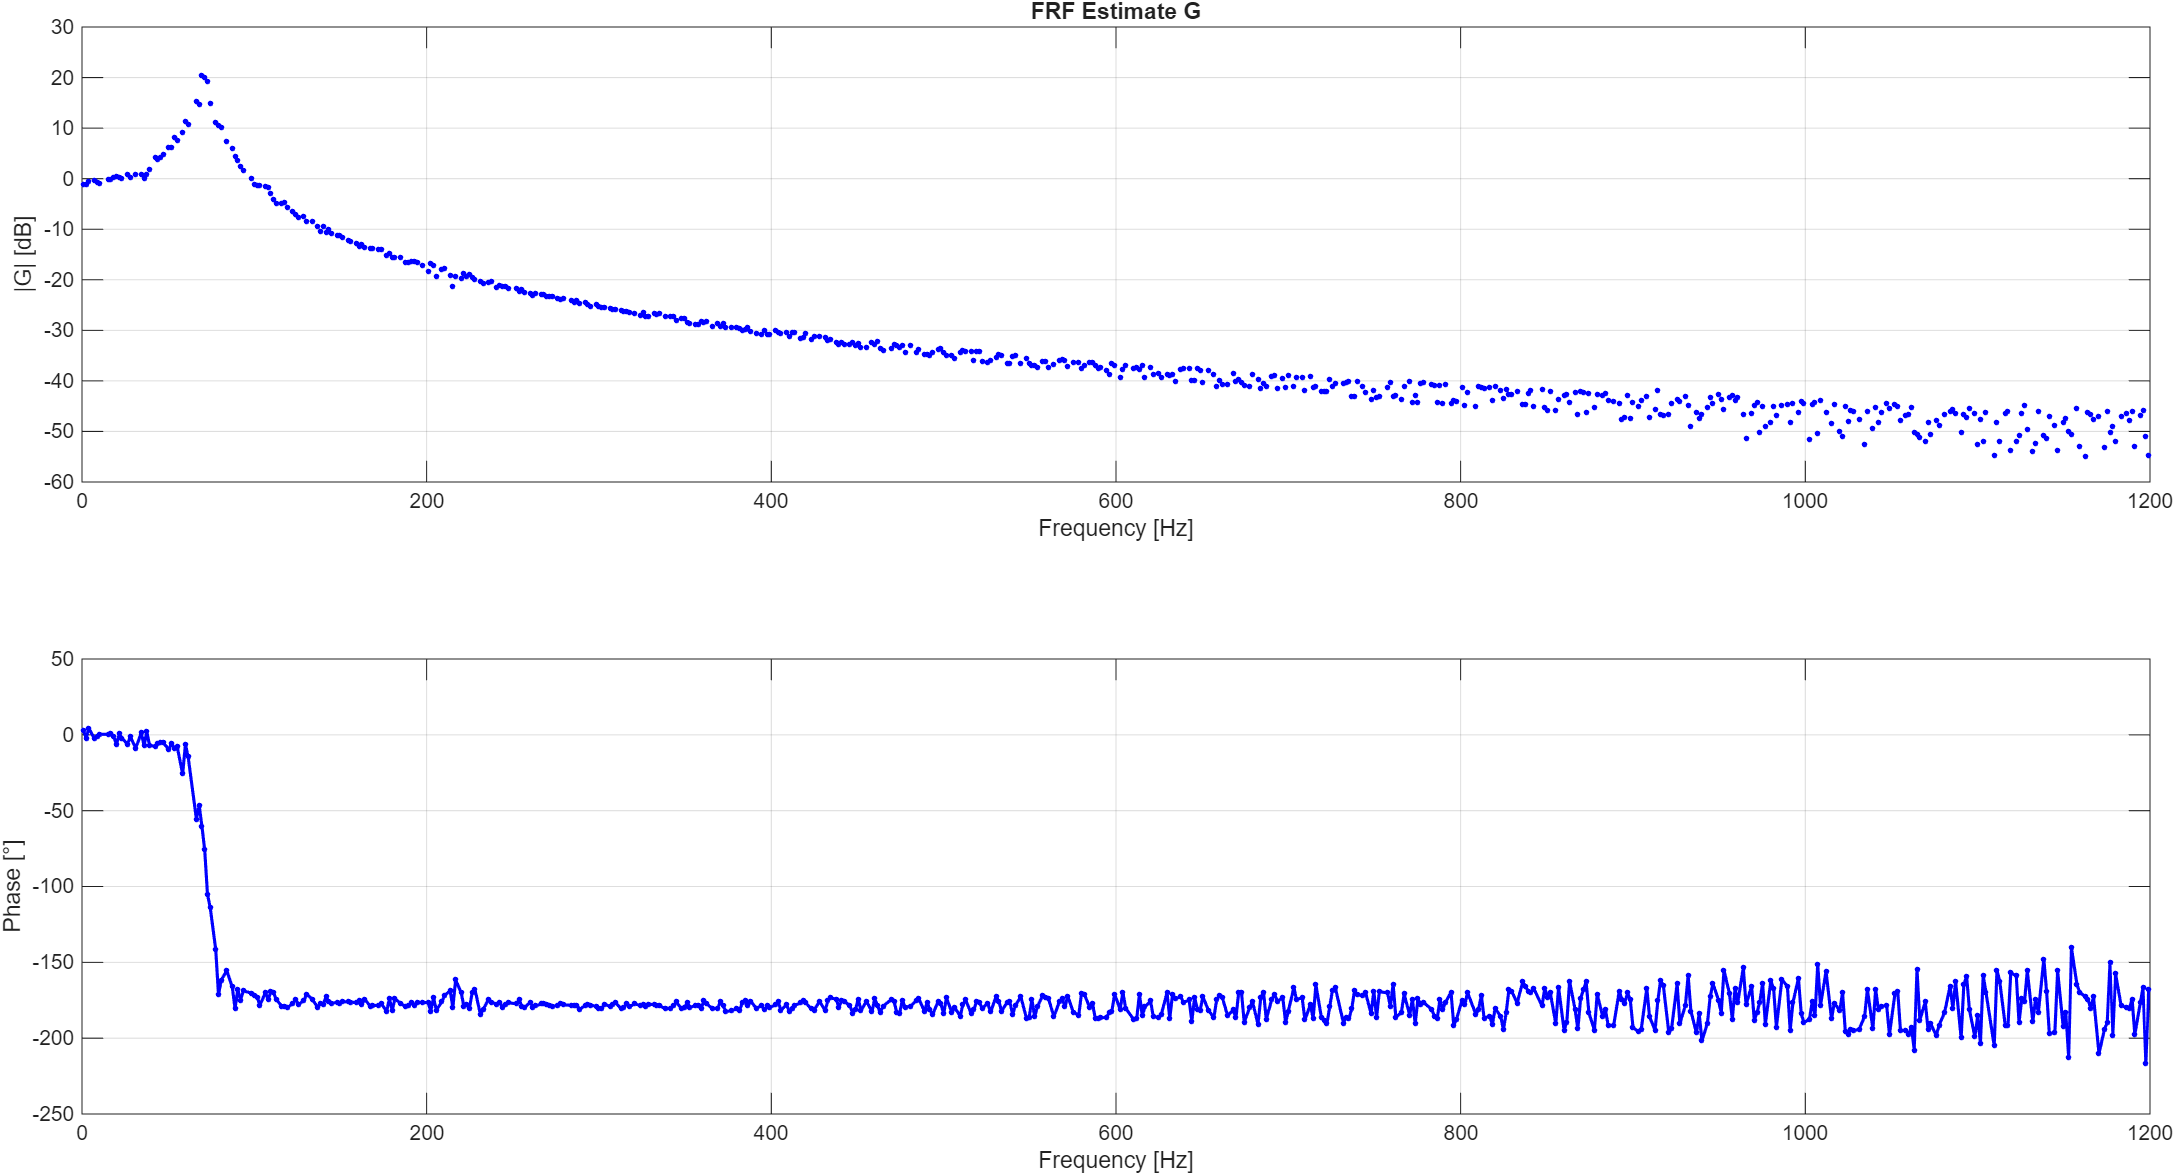
\includegraphics[width=1\textwidth]{pic/2_Fast_Method_Result_G.png}
    \caption{Output spectrum Y using the fast method}
    \label{fig:fast_Y}
\end{figure}

And in Figure~\ref{fig:fast_Y}, we can see the non-parametric FRF estimate using the fast method only computed at the excited frequencies.

\subsection{Robust method}

In the robust method, we can estimate the FRF using multiple realizations. The FRF is estimated at all frequencies in the frequency band of interest. The nonlinear distortions can be estimated by looking at the variance of the output at each frequency over the different realizations. The noise level can be estimated by looking at the variance of $\hat{G}$ at each frequency over the different realizations.

\begin{figure}[H]
    \centering
    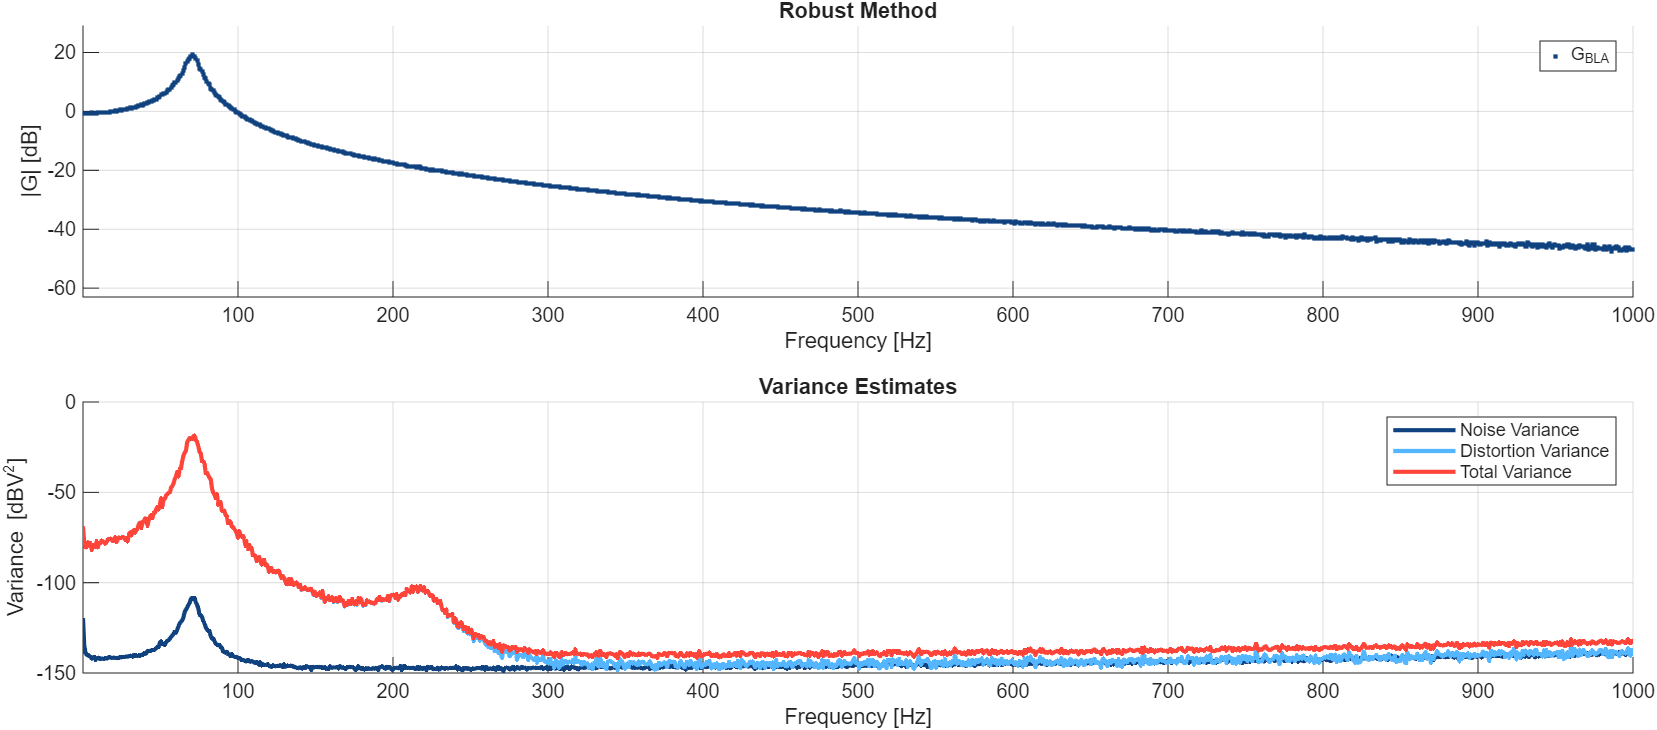
\includegraphics[width=1\textwidth]{pic/2_Robust_Method_Result.png}
    \caption{Non-parametric FRF estimate using the robust method}
    \label{fig:robust_FRF}
\end{figure}

\chapter{Parametric Estimate of the System}

A parametric model can be estimated by fitting a model to the non-parametric FRF estimate. The model can be chosen as a transfer function with a certain number of poles and zeros. The parameters of the model can be estimated using multiple methods.

\section{Transfer Function Model}

We want to estimate a discrete-time transfer function in the z-domain:

\begin{equation}
    G(z) = \frac{B(z)}{A(z)} = \frac{b_0 + b_1 z^{-1} + b_2 z^{-2} + \cdots + b_{n_b} z^{-n_b}}{a_0 + a_1 z^{-1} + a_2 z^{-2} + \cdots + a_{n_a} z^{-n_a}}
    \label{eq:transfer_function}
\end{equation}

The transfer function $G(z)$ is defined up to a scaling factor: multiplying both $B(z)$ and $A(z)$ by a constant does not change $G(z)$. To make the problem identifiable, we need to impose a \textbf{constraint} on the parameters. Two common choices are:

\begin{enumerate}
    \item \textbf{Monic constraint:} Fix the leading coefficient of $A(z)$ to 1, i.e., $a_0 = 1$. This is used in LLS, WLS, and IQML methods.
    \item \textbf{Norm constraint:} Require $\|\theta\|^2 = 1$. This is used in the Total Least Squares (TLS) method.
\end{enumerate}

\subsubsection{Monic Constraint}

With the monic constraint $a_0 = 1$, the parameter vector becomes:

\begin{equation}
    \theta_{\text{monic}} = \begin{bmatrix} b_0 & b_1 & \cdots & b_{n_b} & a_1 & \cdots & a_{n_a} \end{bmatrix}^T
\end{equation}

\subsubsection{Norm Constraint}

With the norm constraint, all coefficients including $a_0$ are estimated:

\begin{equation}
    \theta_{\text{norm}} = \begin{bmatrix} b_0 & b_1 & \cdots & b_{n_b} & a_0 & a_1 & \cdots & a_{n_a} \end{bmatrix}^T, \quad \|\theta_{\text{norm}}\|^2 = 1
\end{equation}

\section{Derivation of the Regressor Matrix}

Starting from the transfer function model in \eqref{eq:transfer_function}, we cross-multiply to obtain:

\begin{equation}
    G(z) \cdot A(z) = B(z)
\end{equation}

Expanding both sides:

\begin{equation}
    G(z) \cdot \left(a_0 + a_1 z^{-1} + \cdots + a_{n_a} z^{-n_a}\right) = b_0 + b_1 z^{-1} + \cdots + b_{n_b} z^{-n_b}
\end{equation}

This can be rewritten as:

\begin{equation}
    b_0 + b_1 z^{-1} + \cdots + b_{n_b} z^{-n_b} - G(z) a_0 - G(z) a_1 z^{-1} - \cdots - G(z) a_{n_a} z^{-n_a} = 0
\end{equation}

\subsubsection{Regressor for Norm Constraint (TLS)}

For Total Least Squares with the norm constraint $\|\theta\|=1$, the regressor row for frequency $z_k$ is:

\begin{equation}
    \phi_k^{\text{TLS}} = \begin{bmatrix} 1 & z_k^{-1} & \cdots & z_k^{-n_b} & -G_k & -G_k z_k^{-1} & \cdots & -G_k z_k^{-n_a} \end{bmatrix}
\end{equation}

The full system becomes $\Phi^{\text{TLS}} \theta = 0$, a homogeneous system.

\subsubsection{Regressor for Monic Constraint (LLS/WLS/IQML)}

With the monic constraint $a_0 = 1$, we rearrange to isolate $G(z)$:

\begin{equation}
    G(z) = b_0 + b_1 z^{-1} + \cdots + b_{n_b} z^{-n_b} - G(z) a_1 z^{-1} - \cdots - G(z) a_{n_a} z^{-n_a}
\end{equation}

For a single frequency point $z_k = e^{j 2\pi f_k / f_s}$, this can be written in matrix form as:

\begin{equation}
    G_k = \underbrace{\begin{bmatrix} 1 & z_k^{-1} & \cdots & z_k^{-n_b} & -G_k z_k^{-1} & \cdots & -G_k z_k^{-n_a} \end{bmatrix}}_{\phi_k} \theta_{\text{monic}}
\end{equation}

For $K$ frequency points, we stack the rows to form the full regressor matrix:

\begin{equation}
    \underbrace{\begin{bmatrix} G_1 \\ G_2 \\ \vdots \\ G_K \end{bmatrix}}_{Y} = \underbrace{\begin{bmatrix} 
    1 & z_1^{-1} & \cdots & z_1^{-n_b} & -G_1 z_1^{-1} & \cdots & -G_1 z_1^{-n_a} \\ 
    1 & z_2^{-1} & \cdots & z_2^{-n_b} & -G_2 z_2^{-1} & \cdots & -G_2 z_2^{-n_a} \\ 
    \vdots & \vdots & \ddots & \vdots & \vdots & \ddots & \vdots \\ 
    1 & z_K^{-1} & \cdots & z_K^{-n_b} & -G_K z_K^{-1} & \cdots & -G_K z_K^{-n_a} 
    \end{bmatrix}}_{\Phi} \theta_{\text{monic}}
    \label{eq:regressor_matrix}
\end{equation}

\section{Handling Complex Data with Real Parameters}

The parameters $(b_0, \ldots, b_{n_b}, a_1, \ldots, a_{n_a})$ are \textbf{real numbers} since we are estimating a transfer function of a real system. However, the regressor matrix $\Phi$ and the measured FRF $G$ are \textbf{complex-valued}.

To enforce real-valued solutions, we convert the complex least squares problem into a real one by stacking the real and imaginary parts:

\begin{equation}
    \Phi \theta = Y \quad \Rightarrow \quad 
    \begin{bmatrix} \text{Re}(\Phi) \\ \text{Im}(\Phi) \end{bmatrix} \theta = 
    \begin{bmatrix} \text{Re}(Y) \\ \text{Im}(Y) \end{bmatrix}
    \label{eq:real_stacking}
\end{equation}

This doubles the number of equations and ensures a real-valued least squares solution.

\section{Linear Least Squares (LLS)}

The simplest approach minimizes the equation error:

\begin{equation}
    \hat{\theta}_{LLS} = \arg\min_\theta \| \Phi \theta - Y \|^2
\end{equation}

Using the real-valued formulation from \eqref{eq:real_stacking}, the solution is:

\begin{equation}
    \hat{\theta}_{LLS} = \left( \Phi_\mathbb{R}^T \Phi_\mathbb{R} \right)^{-1} \Phi_\mathbb{R}^T Y_\mathbb{R}
\end{equation}

where $\Phi_\mathbb{R}$ and $Y_\mathbb{R}$ denote the stacked real and imaginary parts.

\textbf{Limitations of LLS:}
\begin{itemize}
    \item LLS treats all frequency points equally, regardless of the noise level at each frequency.
    \item With uniformly spaced frequency points on a linear scale, higher frequencies contribute disproportionately more to the cost function. For example, between 10--100 Hz there are $\sim$90 frequency bins, but between 100--1000 Hz there are $\sim$900 bins. This causes the estimate to be biased towards fitting high-frequency behavior at the expense of low-frequency accuracy. A possible remedy is to apply logarithmic frequency weighting, i.e., $w_k \propto 1/f_k$.
\end{itemize}

\begin{figure}[H]
    \centering
    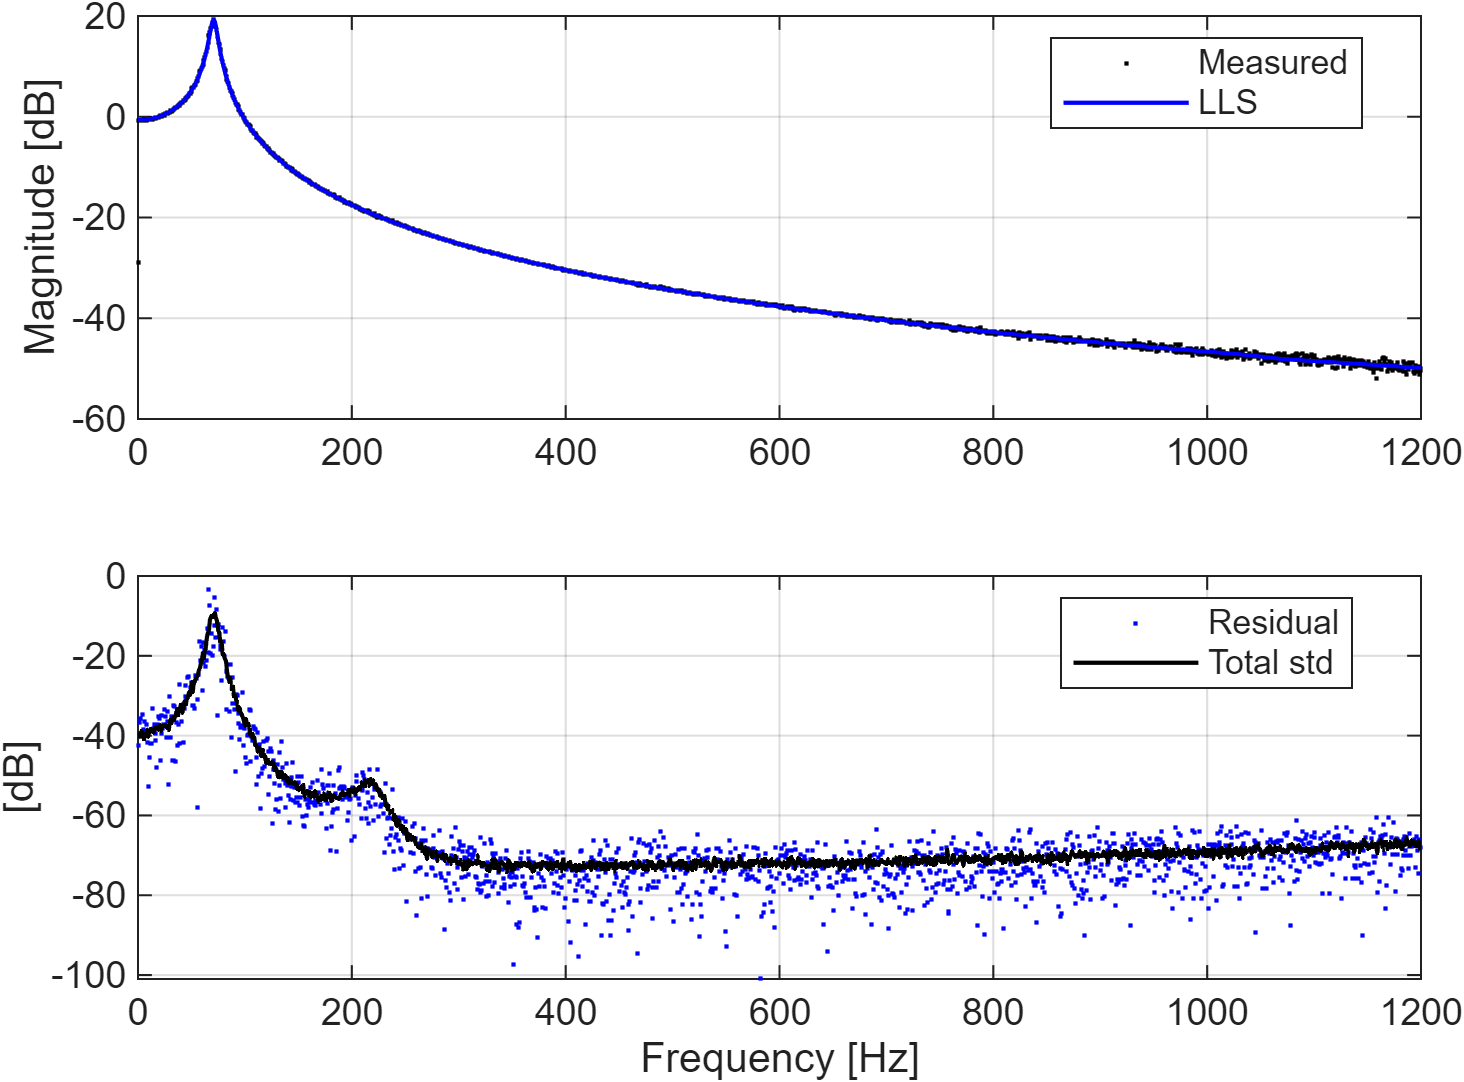
\includegraphics[width=0.8\textwidth]{pic/2_LLS_Fit.png}
    \caption{Parametric model fit using Linear Least Squares (LLS) method}
    \label{fig:lls_fit}
\end{figure}


\section{Iterative Weighted Least Squares (IWLS)}

The IWLS method, also known as the Sanathanan-Koerner algorithm, attempts to correct for the equation error bias without requiring knowledge of the noise variance. The key insight is that minimizing equation error $|A \cdot G - B|^2$ implicitly weights by $|A|^2$, which biases the estimate away from poles.

\subsection{The Sanathanan-Koerner Algorithm}

IWLS iteratively reweights the least squares problem by $1/|A(z)|^2$:

\begin{equation}
    \hat{\theta}_{IWLS}^{(i)} = \arg\min_\theta \sum_{k=1}^{K} \frac{1}{\left|A^{(i-1)}(z_k)\right|^2} \left| \phi_k \theta - G_k \right|^2
\end{equation}

The algorithm proceeds as follows:

\begin{enumerate}
    \item \textbf{Initialize:} Obtain $\hat{\theta}^{(0)}$ using LLS.
    
    \item \textbf{Iterate} for $i = 1, 2, \ldots$:
    \begin{enumerate}
        \item Compute $A^{(i-1)}(z_k)$ from the previous estimate
        \item Set weights $w_k = 1/|A^{(i-1)}(z_k)|^2$
        \item Solve the weighted least squares problem
    \end{enumerate}
    
    \item \textbf{Convergence:} Stop when parameters stabilize.
\end{enumerate}



\begin{figure}[H]
    \centering
    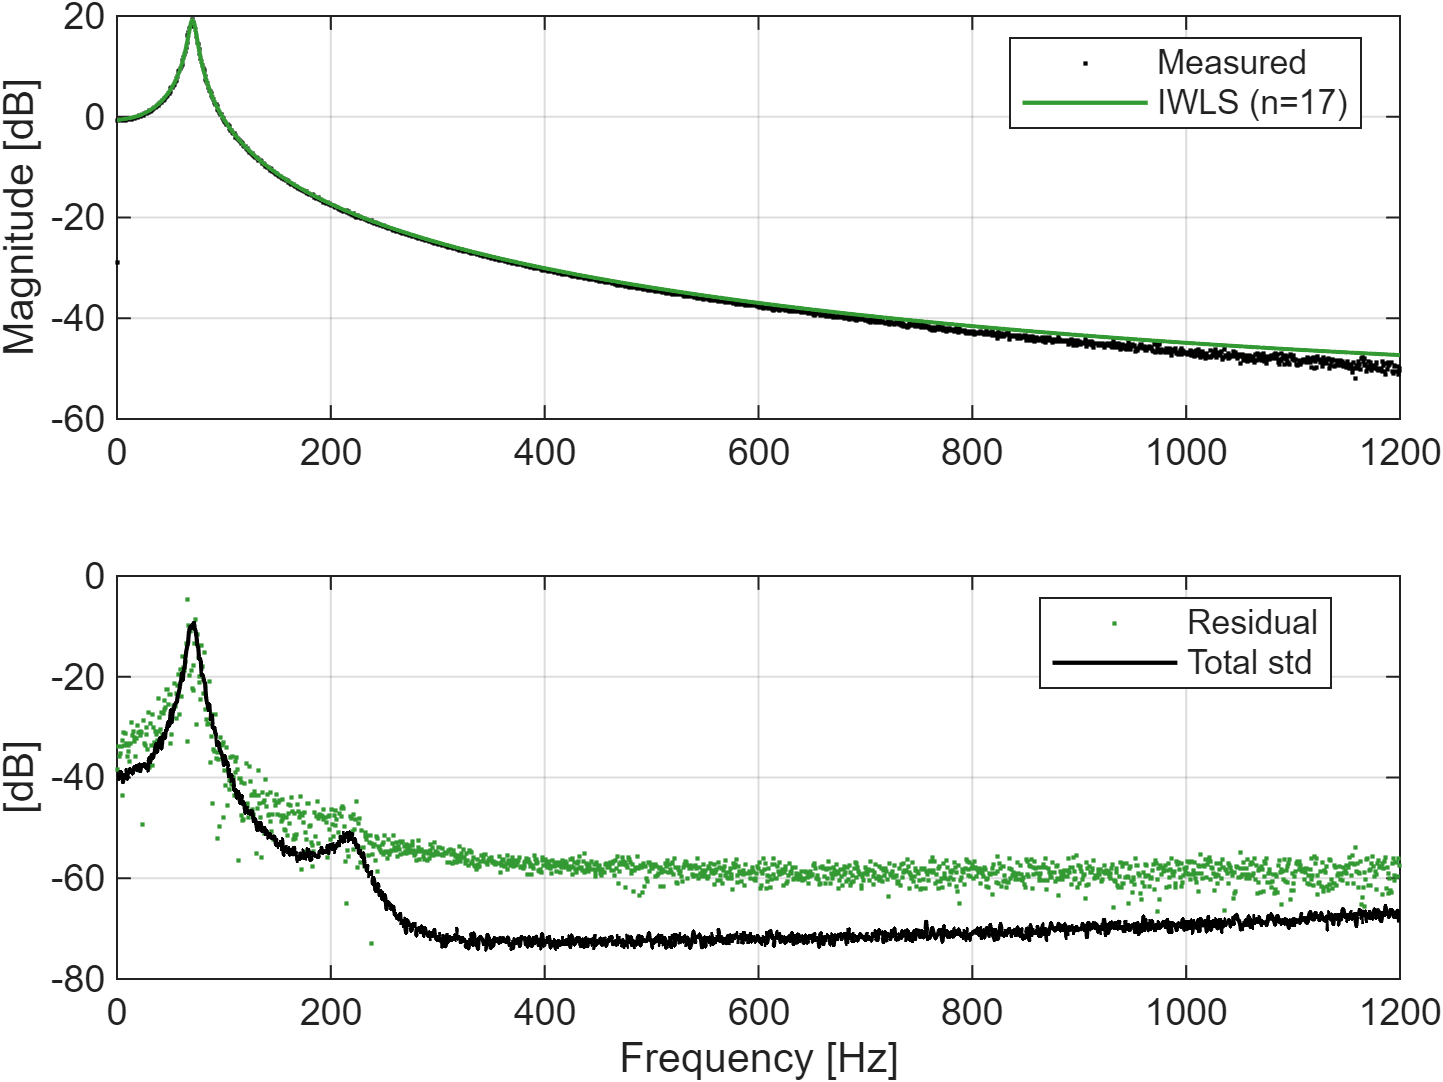
\includegraphics[width=0.8\textwidth]{pic/2_IWLS_Fit.png}
    \caption{Parametric model fit using Iterative Weighted Least Squares (IWLS) method}
    \label{fig:iwls_fit}
\end{figure}


\section{Total Least Squares (TLS)}

The Total Least Squares method uses the norm constraint $\|\theta\|^2 = 1$ instead of the monic constraint.

The equation $\Phi^{\text{TLS}} \theta = 0$ is homogeneous, meaning any scalar multiple of a solution is also a solution. The norm constraint $\|\theta\|^2 = 1$ removes this scaling ambiguity.

The TLS minimizer is:

\begin{equation}
    \hat{\theta}_{TLS} = \arg\min_\theta \frac{\left\| \Phi^{\text{TLS}} \theta \right\|^2}{\|\theta\|^2}
    \label{eq:tls_cost}
\end{equation}

This is equivalent to minimizing $\left\| \Phi^{\text{TLS}} \theta \right\|^2$ subject to the constraint $\|\theta\|^2 = 1$.



\subsubsection{Solution via SVD}

Using the SVD on the real-valued stacked matrix:

\begin{equation}
    \Phi_{\mathbb{R}}^{\text{TLS}} = U \Sigma V^T
\end{equation}

where $\Sigma = \text{diag}(\sigma_1, \sigma_2, \ldots, \sigma_n)$ with $\sigma_1 \geq \sigma_2 \geq \cdots \geq \sigma_n \geq 0$.

The cost function can be written as:

\begin{equation}
    \left\| \Phi_{\mathbb{R}}^{\text{TLS}} \theta \right\|^2 = \left\| U \Sigma V^T \theta \right\|^2 = \left\| \Sigma V^T \theta \right\|^2 = \sum_{i=1}^{n} \sigma_i^2 (v_i^T \theta)^2
\end{equation}

Since $\|\theta\|^2 = 1$ and $V$ is orthonormal, we have $\sum_i (v_i^T \theta)^2 = 1$. To minimize the cost, we should put all weight on the smallest singular value, i.e., choose $\theta = v_n$ (the last column of $V$):

\begin{equation}
    \hat{\theta}_{TLS} = V(:, \text{end})
\end{equation}

The minimum cost achieved is $\sigma_n^2$, the square of the smallest singular value.

\textbf{Advantage:} TLS treats errors in both the numerator and denominator parts symmetrically, which can be beneficial when the FRF measurements have errors.


\begin{figure}[H]
    \centering
    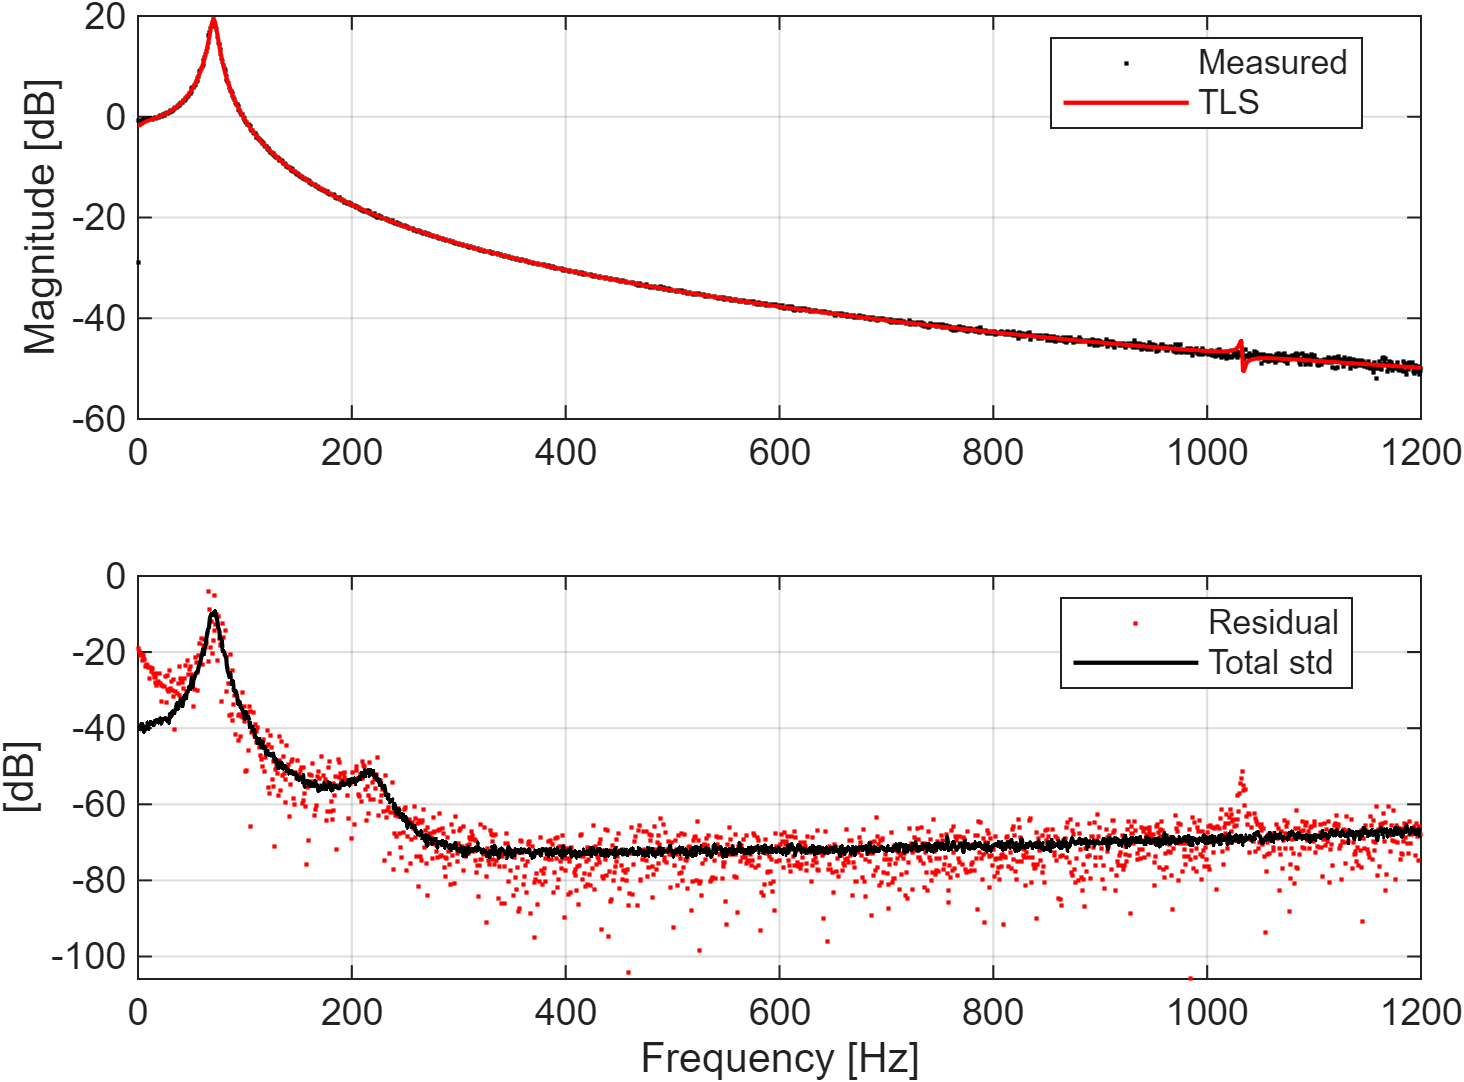
\includegraphics[width=0.8\textwidth]{pic/2_TLS_Fit.png}
    \caption{Parametric model fit using Total Least Squares (TLS) method}
    \label{fig:tls_fit}
\end{figure}



\section{Generalized Total Least Squares (GTLS)}

The TLS method, while elegant, is not consistent: it uses the constraint $\|\theta\|^2 = 1$, which treats all parameters equally and does not account for the heteroscedastic noise (frequency-dependent noise variance $\sigma_k^2$).

The Generalized Total Least Squares (GTLS) method extends TLS by modifying the constraint to incorporate the noise covariance structure. This extension achieves two important properties:
\begin{enumerate}
    \item \textbf{Consistency:} By properly weighting each row according to its noise contribution, GTLS produces asymptotically unbiased estimates.
    \item \textbf{Convexity:} The optimization problem remains convex (quadratic in the parameters), allowing for an efficient closed-form solution via the Generalized SVD.
\end{enumerate}

\subsection{Modified Constraint}

Instead of the TLS constraint $\|\theta\|^2 = 1$, GTLS uses:

\begin{equation}
    \|C_J^{1/2} \theta\|^2 = 1
\end{equation}

where $C_J^{1/2}$ is the square root of the noise covariance structure matrix that captures which parts of the regressor are affected by noise.

\subsection{Construction of $C_J^{1/2}$}

For the homogeneous regressor $J = [Z_b, -G \cdot Z_a]$ where:
\begin{itemize}
    \item $Z_b = [z^0, z^{-1}, \ldots, z^{-n_b}]$ (noise-free numerator terms)
    \item $Z_a = [z^0, z^{-1}, \ldots, z^{-n_a}]$ (noise-free denominator frequency terms)
\end{itemize}

The noise only affects the columns multiplied by $G_k$. For each frequency $k$, the noise contribution to row $k$ of the regressor is:

\begin{equation}
    \Delta J_k = [0, \ldots, 0, -\Delta G_k \cdot z_k^0, -\Delta G_k \cdot z_k^{-1}, \ldots, -\Delta G_k \cdot z_k^{-n_a}]
\end{equation}

The square root of the covariance structure matrix $C_J^{1/2}$ is constructed as:

\begin{equation}
    C_J^{1/2}(k,:) = \sigma_k^{1/2} \cdot [0, \ldots, 0, z_k^0, z_k^{-1}, \ldots, z_k^{-n_a}]
\end{equation}

where $\sigma_k = \sqrt{\text{var}(G_k)}$ is the noise standard deviation at frequency $k$.

\subsection{Solution via Generalized SVD}

The GTLS problem becomes:

\begin{equation}
    \hat{\theta}_{GTLS} = \arg\min_\theta \|J \theta\|^2
\end{equation}

This is solved using the Generalized Singular Value Decomposition (GSVD). The GSVD of the matrix pair $(J_{\mathbb{R}}, C_{J,\mathbb{R}}^{1/2})$ gives:

\begin{align}
    J_{\mathbb{R}} &= U \cdot C \cdot X^T \\
    C_{J,\mathbb{R}}^{1/2} &= V \cdot S \cdot X^T
\end{align}

where $C$ and $S$ are diagonal matrices satisfying $C^T C + S^T S = I$.

The generalized singular values are:

\begin{equation}
    \gamma_i = \frac{C_{ii}}{S_{ii}}
\end{equation}

The GTLS solution is:

\begin{equation}
    \hat{\theta}_{GTLS} = \frac{X^{-T}(:, i_{\min})}{S_{i_{\min}, i_{\min}}}
\end{equation}

where $i_{\min} = \arg\min_i \gamma_i$ corresponds to the smallest generalized singular value.

\begin{figure}[H]
    \centering
    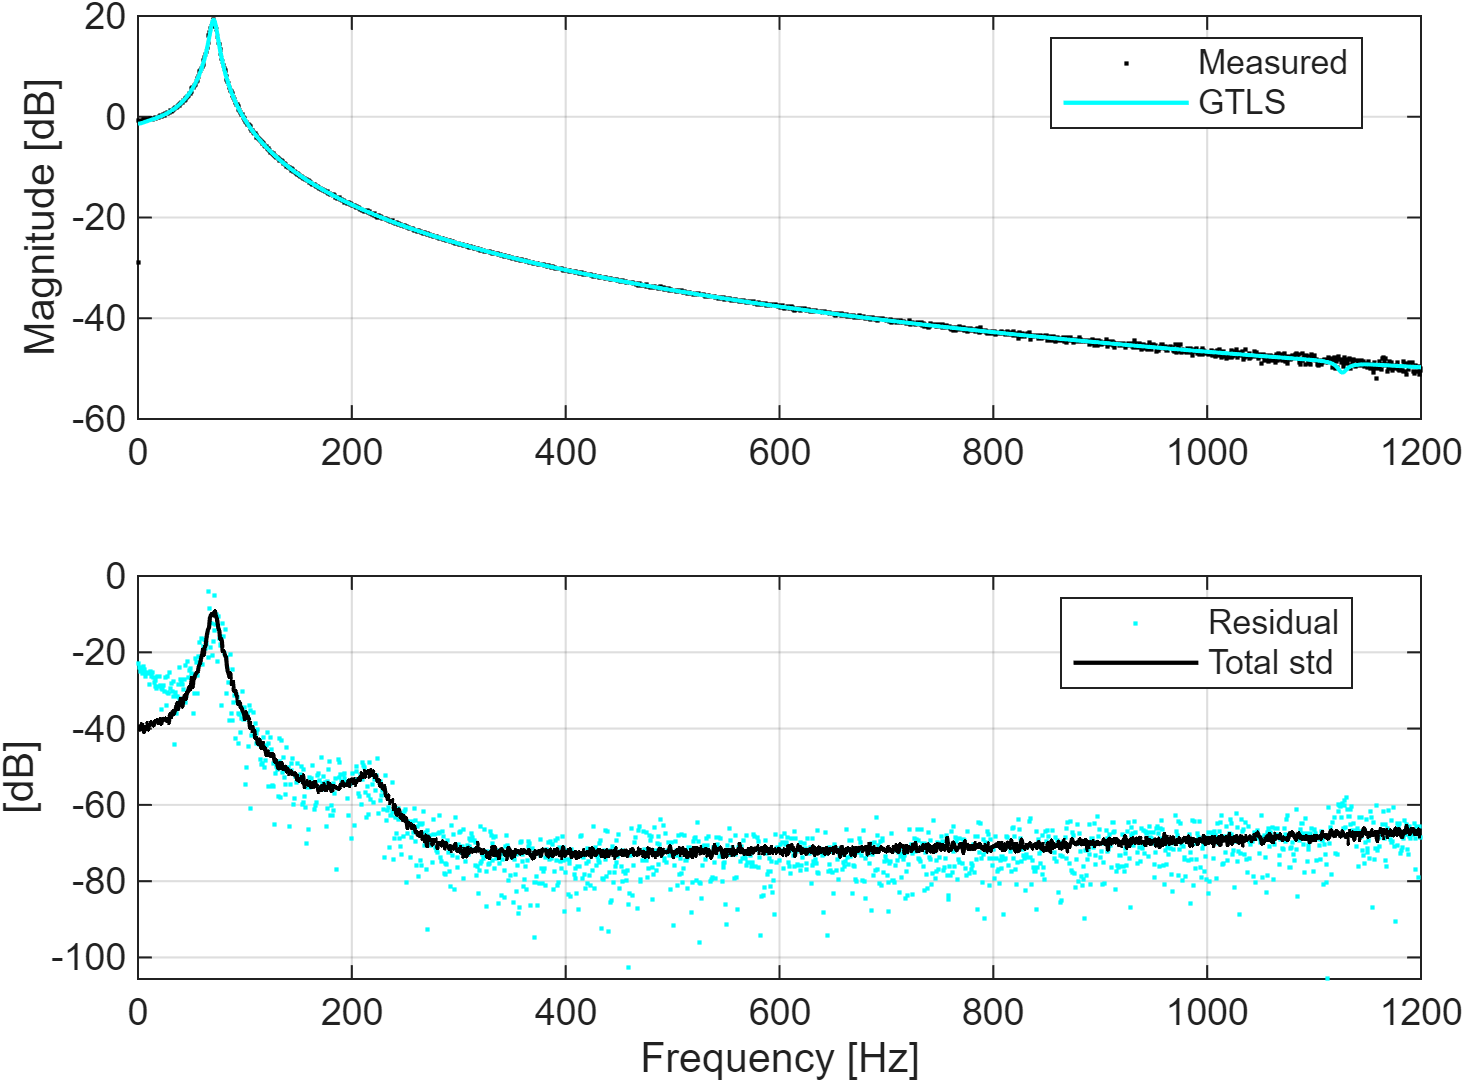
\includegraphics[width=0.8\textwidth]{pic/2_GTLS_Fit.png}
    \caption{Parametric model fit using Generalized Total Least Squares (GTLS) method}
    \label{fig:gtls_fit}
\end{figure}


\section{Weighted Least Squares (WLS)}

When the noise variance $\sigma_k^2$ at each frequency is known (from the non-parametric estimation), we can weight each frequency accordingly:

\begin{equation}
    \hat{\theta}_{WLS} = \arg\min_\theta \sum_{k=1}^{K} \frac{1}{\sigma_k^2} \left| \phi_k \theta - G_k \right|^2
\end{equation}

This is solved by defining the weight matrix (with $K$ the number of frequency points):

\begin{equation}
    W = \text{diag}\left(\frac{1}{\sigma_1}, \frac{1}{\sigma_2}, \ldots, \frac{1}{\sigma_K}\right)
\end{equation}

The solution becomes:

\begin{equation}
    \hat{\theta}_{WLS} = (W\Phi)^\dagger (WY)
\end{equation}

\textbf{Advantage:} Frequencies with lower noise receive higher weight, so more reliable data contributes more to the estimate.

\begin{figure}[H]
    \centering
    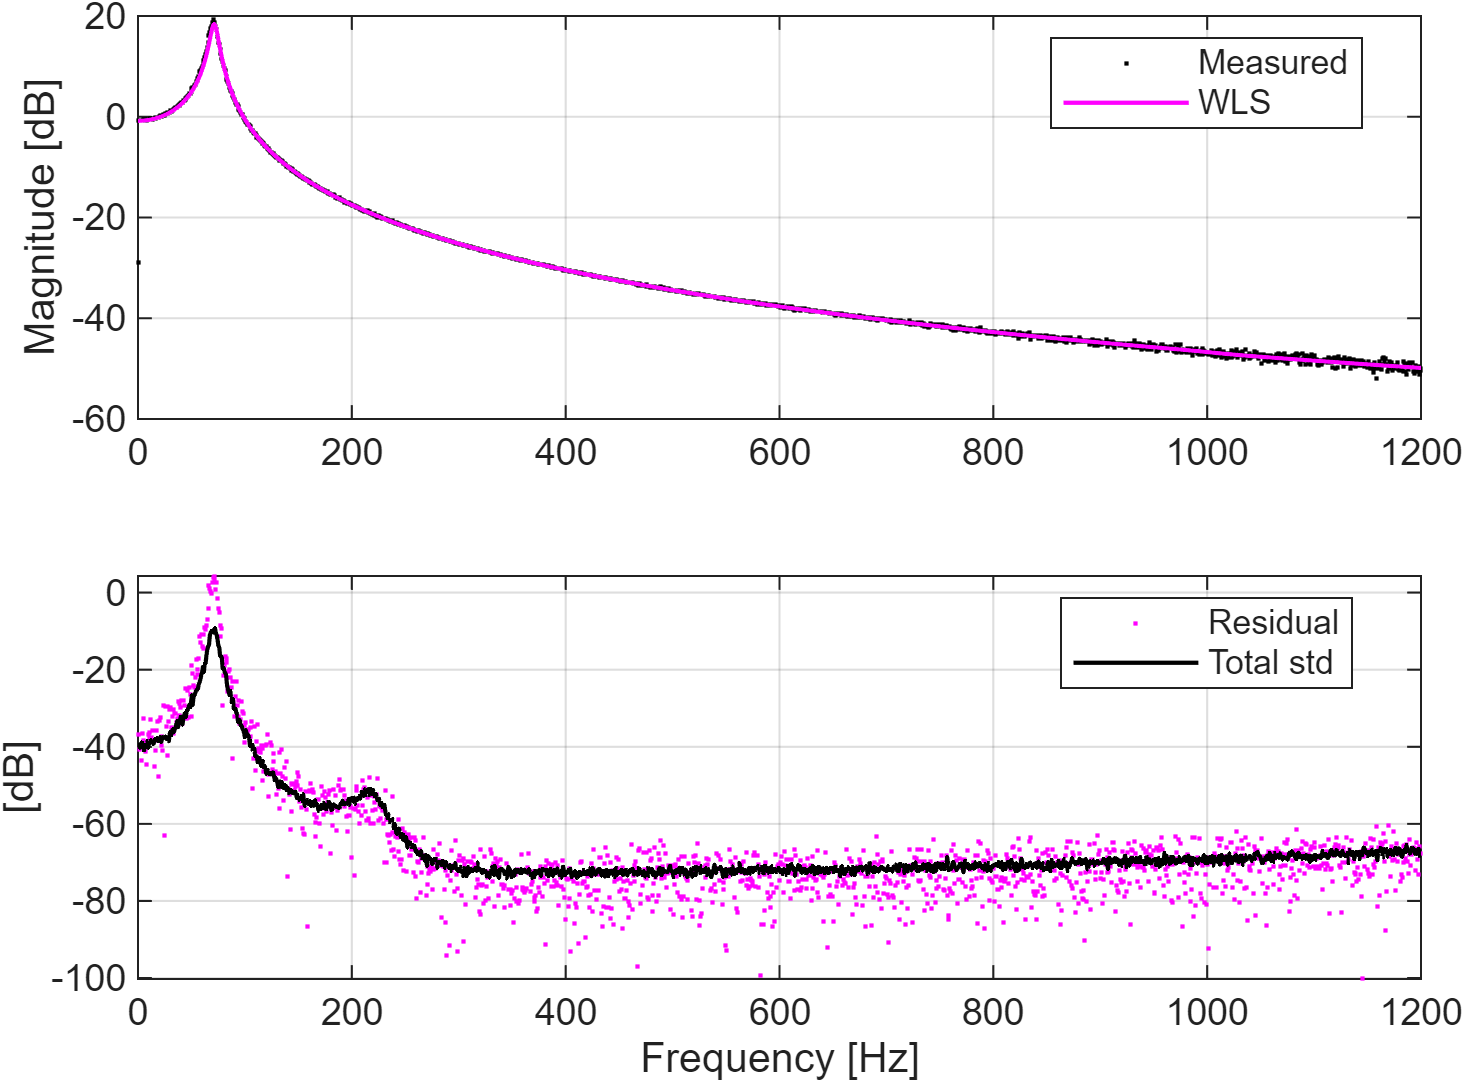
\includegraphics[width=0.8\textwidth]{pic/2_WLS_Fit.png}
    \caption{Parametric model fit using Weighted Least Squares (WLS) method}
    \label{fig:wls_fit}
\end{figure}



\section{Iterative Quadratic Maximum Likelihood (IQML)}

\subsection{The Problem with Equation Error}

Both LLS and WLS minimize the \textbf{equation error}:

\begin{equation}
    \varepsilon_{EQ} = G \cdot A(z) - B(z)
\end{equation}

However, what we really want to minimize is the \textbf{output error}:

\begin{equation}
    \varepsilon_{OUT} = G - \frac{B(z)}{A(z)}
\end{equation}

The relationship between these two errors is:

\begin{equation}
    \varepsilon_{EQ} = G \cdot A(z) - B(z) = A(z) \cdot \left( G - \frac{B(z)}{A(z)} \right) = A(z) \cdot \varepsilon_{OUT}
\end{equation}

This means the equation error is scaled by $|A(z)|$, which introduces a \textbf{bias} in the estimate. Near the poles of the system (where $|A(z)|$ is small), the equation error underweights those frequencies.

\subsection{Correcting for the Equation Error Bias}

To properly minimize the output error, we need to weight by $\frac{1}{|A(z)|^2}$. However, instead of using the full weighting, IQML uses a parameter $r \in [0, 1]$ that controls the weighting strength:

\begin{equation}
    \hat{\theta}_{IQML}^{(i)} = \arg\min_\theta \sum_{k=1}^{K} \frac{\left| \phi_k \theta - G_k \right|^2}{\sigma_{e,k}^{2r}}
    \label{eq:iqml_cost}
\end{equation}

where $\sigma_{e,k}^2$ is the \textbf{equation error variance} at frequency $k$:

\begin{equation}
    \sigma_{e,k}^2 = \sigma_k^2 \cdot \left|A^{(i-1)}(z_k)\right|^2
    \label{eq:equation_error_variance}
\end{equation}

This relationship follows from $\varepsilon_{EQ} = A \cdot \varepsilon_{OUT}$, so the variance scales by $|A|^2$.

The parameter $r$ provides a trade-off:
\begin{itemize}
    \item $r = 1$: Closest resemblance to the Maximum Likelihood estimator
    \item $r = 0$: Equivalent to LLS (no iterative reweighting)
    \item Smaller $r$: Results in a more convex optimization landscape, improving convergence
\end{itemize}

Typically $r = 1$ is chosen to obtain the ML estimate.

\textbf{The challenge:} $A(z)$ depends on $\theta$, which is exactly what we are trying to estimate! This creates a nonlinear optimization problem.

\subsection{Iterative Solution}

The IQML method solves this by iterating:

\begin{enumerate}
    \item \textbf{Initialize:} Obtain an initial estimate $\hat{\theta}^{(0)}$ using LLS.
    
    \item \textbf{Iterate} for $i = 1, 2, \ldots$:
    \begin{enumerate}
        \item Compute the denominator polynomial at all frequencies using the previous estimate:
        \begin{equation}
            A^{(i-1)}(z_k) = 1 + a_1^{(i-1)} z_k^{-1} + \cdots + a_{n_a}^{(i-1)} z_k^{-n_a}
        \end{equation}
        
        \item Compute the equation error variance at each frequency:
        \begin{equation}
            \sigma_{e,k}^2 = \sigma_k^2 \cdot \left|A^{(i-1)}(z_k)\right|^2
        \end{equation}
        
        \item Update the weights using the parameter $r$:
        \begin{equation}
            w_k^{(i)} = \frac{1}{\left(\sigma_{e,k}^2\right)^r} = \frac{1}{\sigma_k^{2r} \left|A^{(i-1)}(z_k)\right|^{2r}}
        \end{equation}
        
        \item Solve the weighted least squares problem with the updated weights:
        \begin{equation}
            \hat{\theta}^{(i)} = \arg\min_\theta \sum_{k=1}^{K} w_k^{(i)} \left| \phi_k \theta - G_k \right|^2
        \end{equation}
    \end{enumerate}
    
    \item \textbf{Convergence check:} Stop when:
    \begin{equation}
        \frac{\left\|\theta^{(i)} - \theta^{(i-1)}\right\|}{\left\|\theta^{(i-1)}\right\|} < \epsilon
    \end{equation}
    where $\epsilon$ is a small tolerance (e.g., $10^{-8}$).
\end{enumerate}

\textbf{Advantage:} With $r=1$, IQML has the closest resemblance to the Maximum Likelihood estimator at convergence, it minimizes the same weighted output error cost function. Using $r < 1$ results in a more convex optimization landscape, which can improve convergence when the initial estimate is poor.

\begin{figure}[H]
    \centering
    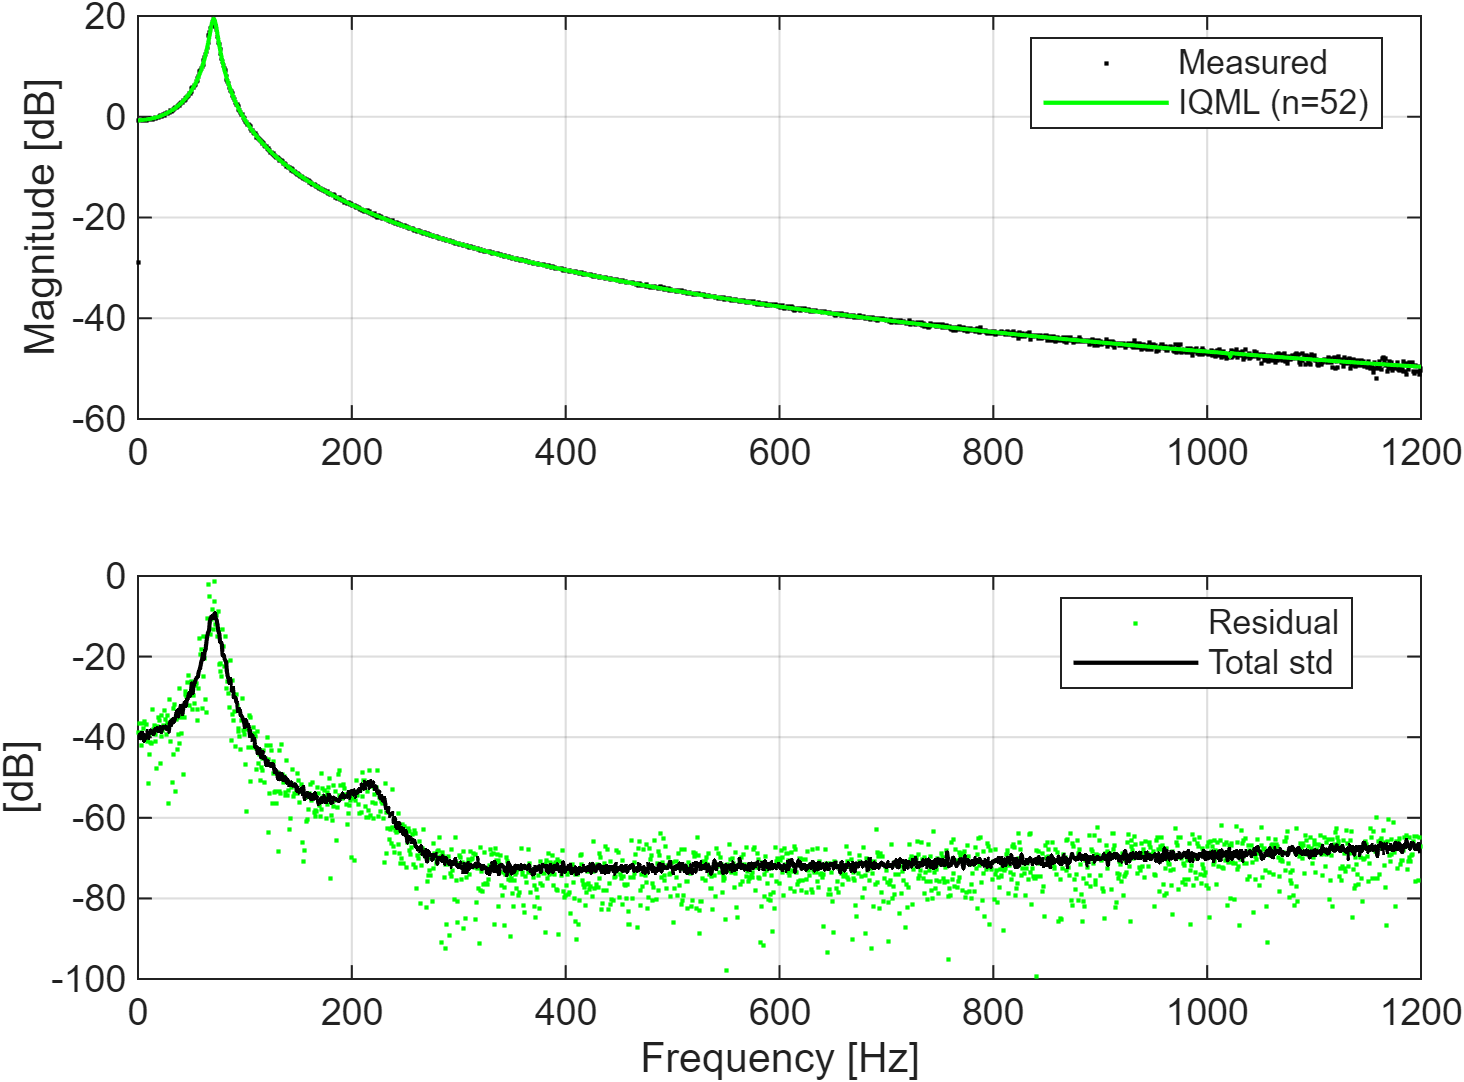
\includegraphics[width=0.8\textwidth]{pic/2_IQML_Fit.png}
    \caption{Parametric model fit using Iterative Quadratic Maximum Likelihood (IQML) method}
    \label{fig:iqml_fit}
\end{figure}



\section{Nonlinear Least Squares via Levenberg-Marquardt (NLS/ML)}

While IQML \emph{approximates} the Maximum Likelihood estimate by iteratively re-weighting the equation error, a more direct approach is to minimize the \textbf{output error} explicitly using nonlinear optimization. The Levenberg-Marquardt algorithm provides robust convergence by blending Gauss-Newton (fast near the optimum) with gradient descent (robust far from the optimum).

\subsection{Output Error Cost Function}

The ML estimator minimizes the weighted output error:

\begin{equation}
    \hat{\theta}_{ML} = \arg\min_{\|\theta\|=1} \sum_{k=1}^{K} \frac{1}{\sigma_k^2} \left| G_k - \frac{B(z_k)}{A(z_k)} \right|^2
\end{equation}

where $\sigma_k$ is the noise standard deviation at frequency $k$. The parameter vector uses \textbf{full parameterization}:
\begin{equation}
    \theta = [b_0, b_1, \ldots, b_{n_b}, a_0, a_1, \ldots, a_{n_a}]^T
\end{equation}
with the constraint $\|\theta\| = 1$ (norm constraint instead of monic). After optimization, the coefficients are normalized so that $a_0 = 1$ for output consistency.

\subsection{Levenberg-Marquardt Optimization}

Define the weighted output error at each frequency:

\begin{equation}
    \varepsilon_k(\theta) = \frac{1}{\sigma_k}\left(G_k - \frac{B(z_k)}{A(z_k)}\right)
\end{equation}

The weighted Jacobian $J_w$ contains the partial derivatives:

\begin{align}
    \frac{\partial \varepsilon}{\partial b_i} &= -\frac{z^{-i}}{\sigma_k \cdot A(z)} \\
    \frac{\partial \varepsilon}{\partial a_j} &= \frac{G_{model} \cdot z^{-j}}{\sigma_k \cdot A(z)}
\end{align}

Using the SVD of the weighted Jacobian $J_w = U \Sigma V^H$, the Levenberg-Marquardt update has the closed-form solution:

\begin{equation}
    \Delta\theta = -V \left(\Sigma^2 + \lambda^2 I\right)^{-1} \Sigma U^H \varepsilon
\end{equation}

where $\lambda$ is the damping parameter:
\begin{itemize}
    \item Large $\lambda$: Behaves like gradient descent (small, safe steps)
    \item Small $\lambda$: Behaves like Gauss-Newton (fast convergence near optimum)
\end{itemize}

\subsection{Algorithm}

\begin{enumerate}
    \item \textbf{Initialize:} Use TLS solution (which already satisfies $\|\theta\|=1$).
    
    \item \textbf{Initialize $\lambda$:} Set $\lambda = 10^{-3} \cdot \sigma_{\max}(J_w)$.
    
    \item \textbf{Iterate} for $i = 1, 2, \ldots$:
    \begin{enumerate}
        \item Compute weighted error $\varepsilon_w$ and weighted Jacobian $J_w$
        
        \item Compute SVD: $J_w = U \Sigma V^H$
        
        \item Compute update: $\Delta\theta = -V (\Sigma^2 + \lambda^2 I)^{-1} \Sigma U^H \varepsilon_w$
        
        \item Try step: $\theta_{try} = (\theta + \Delta\theta) / \|\theta + \Delta\theta\|$
        
        \item If cost decreases: accept step, decrease $\lambda$ by factor 10
        
        \item If cost increases: reject step, increase $\lambda$ by factor 10, retry
    \end{enumerate}
    
    \item \textbf{Convergence:} Stop when $\|\Delta\theta\| / \|\theta\| < 10^{-12}$.
\end{enumerate}




\begin{figure}[H]
    \centering
    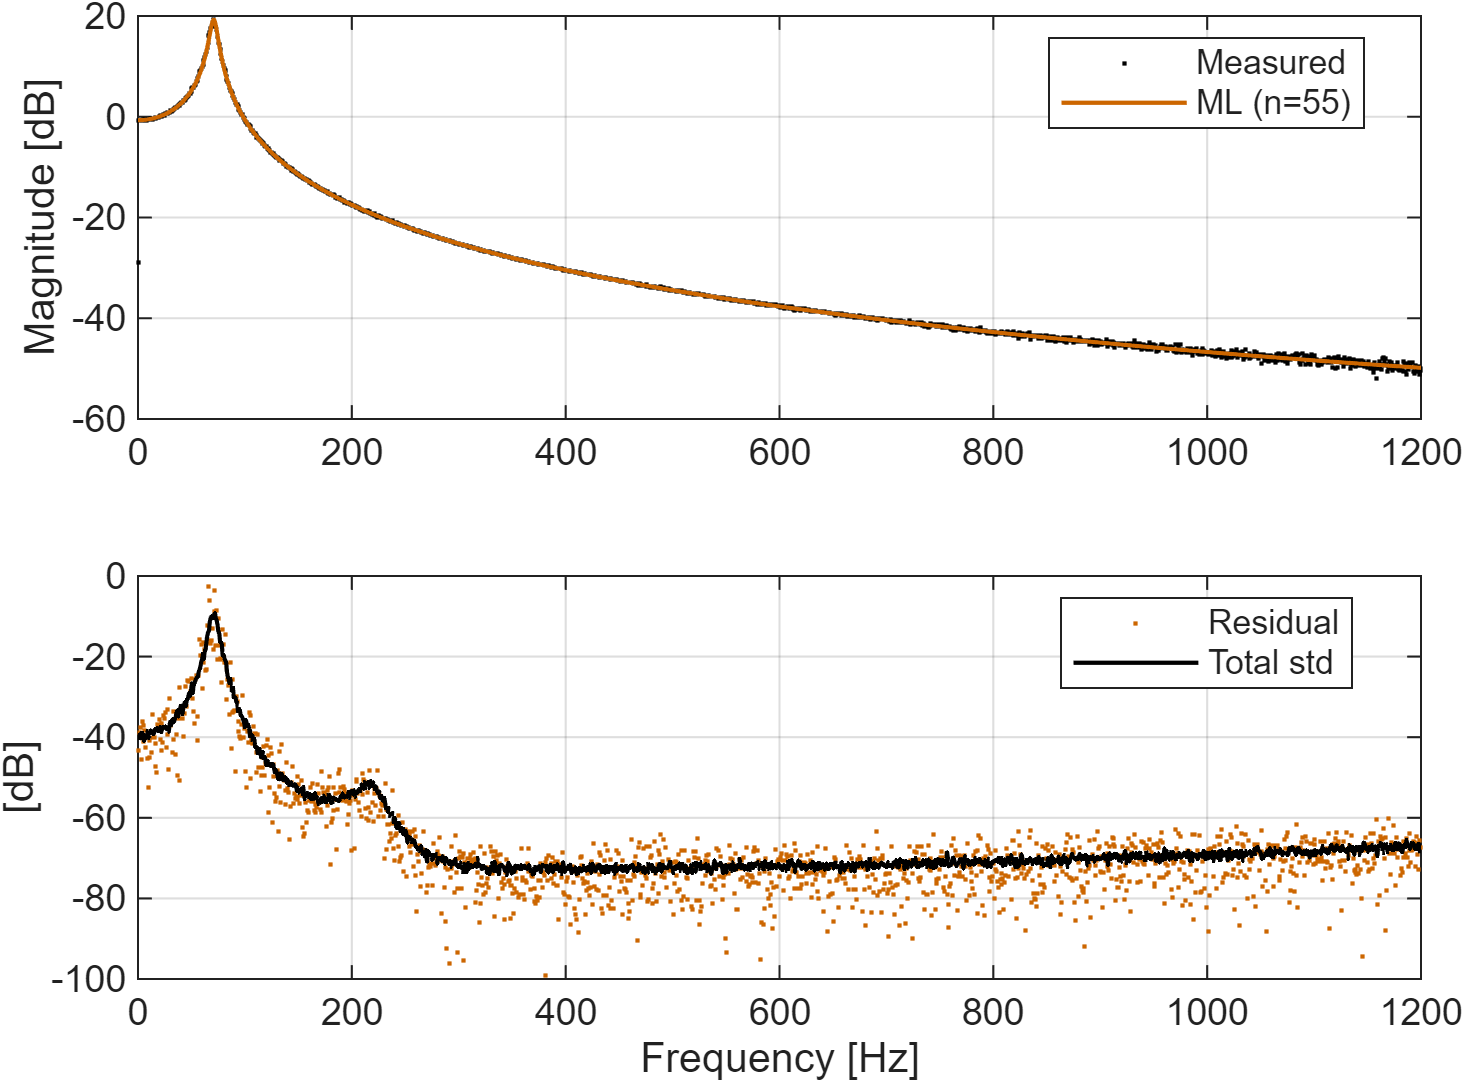
\includegraphics[width=0.8\textwidth]{pic/2_ML_Fit.png}
    \caption{Parametric model fit using Maximum Likelihood via Levenberg-Marquardt}
    \label{fig:ml_fit}
\end{figure}



\section{Summary of Methods}

\begin{table}[H]
\centering
\begin{tabular}{|l|l|l|}
\hline
\textbf{Method} & \textbf{Constraint} & \textbf{Weights $w_k$} \\
\hline
LLS & $a_0=1$ & $1$ \\
\hline
IWLS & $a_0=1$ & $\frac{1}{|A(z_k)|^2}$ (iterative, no noise info) \\
\hline
TLS & $\|\theta\|=1$ & $1$ \\
\hline
GTLS & $\|C_J^{1/2}\theta\|=1$ & $1$ \\
\hline
WLS & $a_0=1$ & $\frac{1}{\sigma_k^2}$ \\
\hline
IQML & $a_0=1$ & $\frac{1}{\sigma_k^2 |A(z_k)|^2}$ (iterative) \\
\hline
ML & $\|\theta\|=1$ & $\frac{1}{\sigma_k^2}$ (Levenberg-Marquardt on output error) \\
\hline
\end{tabular}
\caption{Comparison of parametric estimation methods}
\label{tab:method_comparison}
\end{table}

\subsection{Cost Functions for Comparison}

To compare the quality of the different parametric estimates, we use two cost functions:

\textbf{Weighted cost:}
\begin{equation}
    J_{\text{weighted}} = \sum_{k=1}^{K} \frac{\left| \hat{G}_{\text{ML}}(f_k) - \hat{G}_{\text{model}}(f_k) \right|^2}{\sigma_k^2}
    \label{eq:weighted_cost}
\end{equation}

\textbf{Unweighted cost (raw output error):}
\begin{equation}
    J_{\text{unweighted}} = \sum_{k=1}^{K} \left| \hat{G}_{\text{ML}}(f_k) - \hat{G}_{\text{model}}(f_k) \right|^2
    \label{eq:unweighted_cost}
\end{equation}

where $\hat{G}_{\text{ML}}$ is the non-parametric FRF estimate from the robust method and $\sigma_k^2$ is the total variance (noise + stochastic nonlinear distortion) at frequency $f_k$.

\begin{figure}[H]
    \centering
    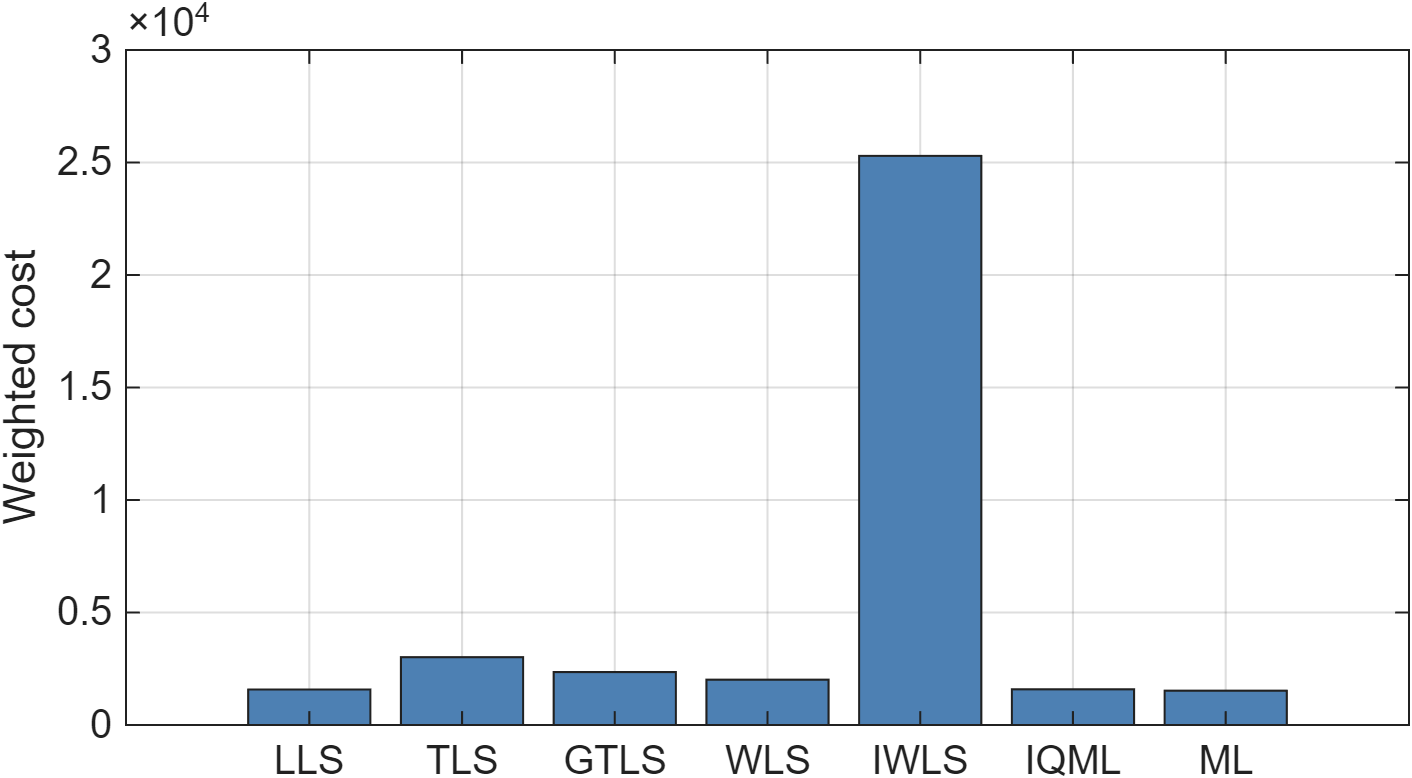
\includegraphics[width=0.48\textwidth]{pic/2_Cost_Comparison.png}
    \hfill
    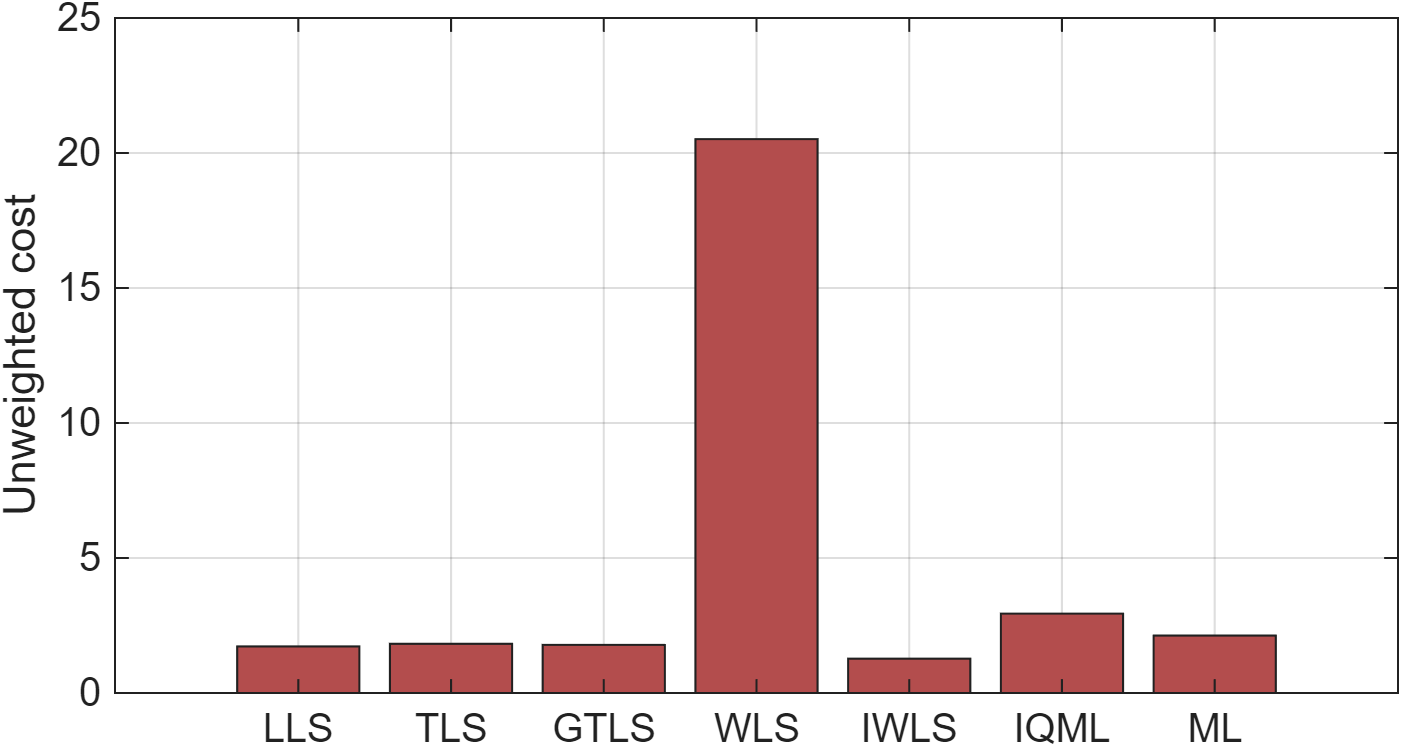
\includegraphics[width=0.48\textwidth]{pic/2_Cost_Comparison_Unweighted.png}
    \caption{Cost comparison across parametric estimation methods. Left: weighted cost $J_{\text{weighted}}$. Right: unweighted cost $J_{\text{unweighted}}$.}
    \label{fig:cost_comparison}
\end{figure}

Note that IWLS is an outlier in the weighted cost (due to overfitting noisy resonances) and WLS is an outlier in the unweighted cost (due to double-weighting: implicit $|A|^2$ combined with explicit $1/\sigma^2$). Figure~\ref{fig:cost_comparison_zoomed} shows the same comparison with these outliers removed for better visualization of the remaining methods.

\begin{figure}[H]
    \centering
    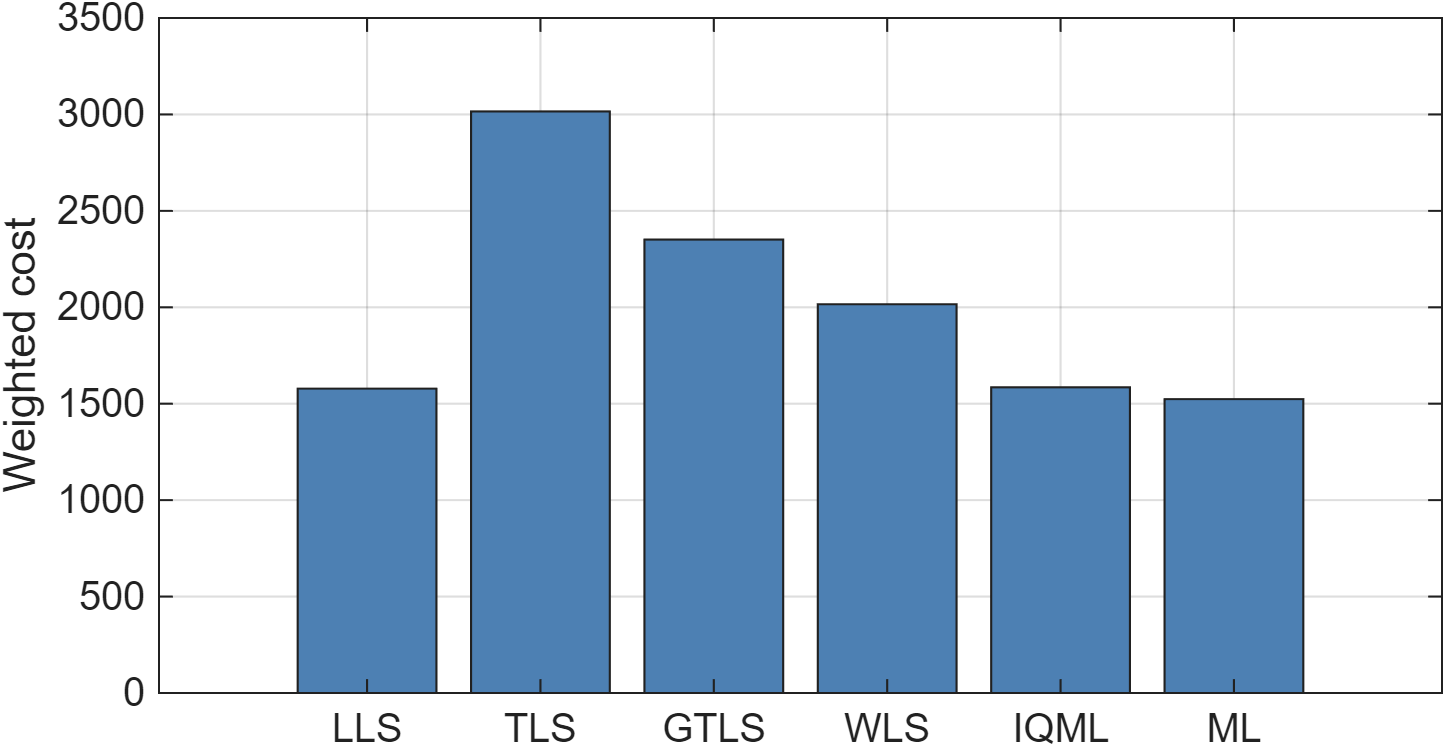
\includegraphics[width=0.48\textwidth]{pic/2_Cost_Comparison_NoIWLS.png}
    \hfill
    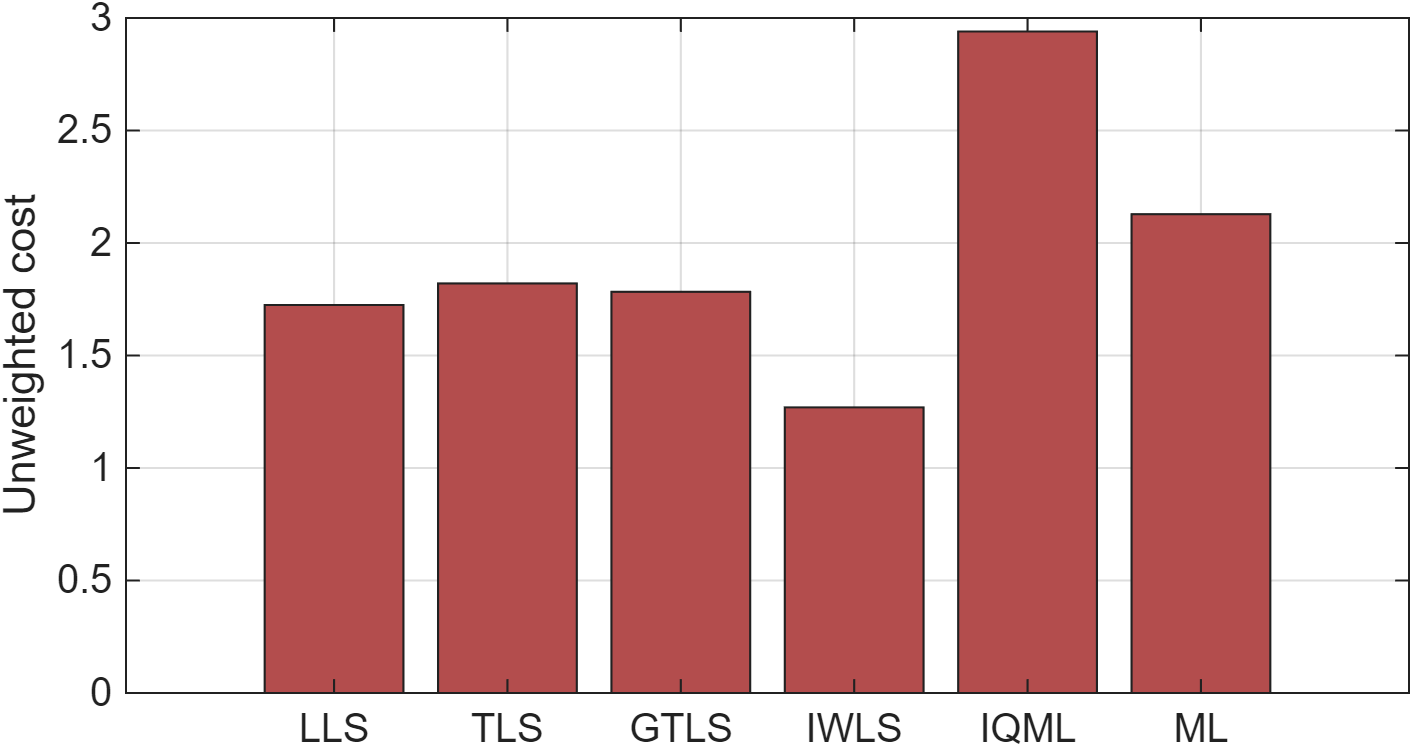
\includegraphics[width=0.48\textwidth]{pic/2_Cost_Comparison_Unweighted_NoWLS.png}
    \caption{Cost comparison with outliers removed. Left: weighted cost without IWLS. Right: unweighted cost without WLS.}
    \label{fig:cost_comparison_zoomed}
\end{figure}

\textbf{Note on model order selection bias:} The model order $(n_a, n_b)$ used in this comparison was selected to be optimal for IQML (see Chapter~\ref{chap:model_order}). This introduces a slight bias in favor of IQML, since LLS, TLS, and WLS might perform relatively better at their own optimal model orders. However, since IQML provides the most statistically sound estimates, using its optimal order for comparison is a reasonable choice.

\subsection{Why Does LLS Perform Well Despite No Noise Weighting?}

A surprising observation is that LLS achieves nearly the same weighted cost as IQML, despite not using any noise information. Meanwhile, IWLS, which explicitly minimizes unweighted output error, performs much worse on the weighted cost.

An explanation could lie in the \textbf{implicit weighting} of LLS. The equation error minimized by LLS is:
\begin{equation}
    \varepsilon_{\text{EQ}} = A(z) \cdot G - B(z) = A(z) \cdot \varepsilon_{\text{OUT}}
\end{equation}

This means LLS implicitly weights each frequency by $|A(z)|^2$. For this system, $|A(z)|^2$ and the total variance $\sigma_k^2$ are \textbf{strongly inversely correlated}:
\begin{equation}
    \text{corr}\left(\log|A(z)|^2, \log \sigma_k^2\right) \approx -0.93
\end{equation}

This correlation arises because:
\begin{itemize}
    \item Near resonances (poles), $|A(z)|$ is small and $|G(z)|$ is large
    \item Stochastic nonlinear distortion scales with output amplitude, so $\sigma_k^2$ is large near resonances
    \item Therefore, $|A(z)|^2 \approx c/\sigma_k^2$ for some constant $c$
\end{itemize}

This means LLS's implicit weighting by $|A(z)|^2$ is approximately equivalent to weighting by $1/\sigma_k^2$: precisely the optimal noise weighting! LLS ``accidentally'' de-emphasizes the high-variance frequencies near resonances.

\begin{figure}[H]
    \centering
    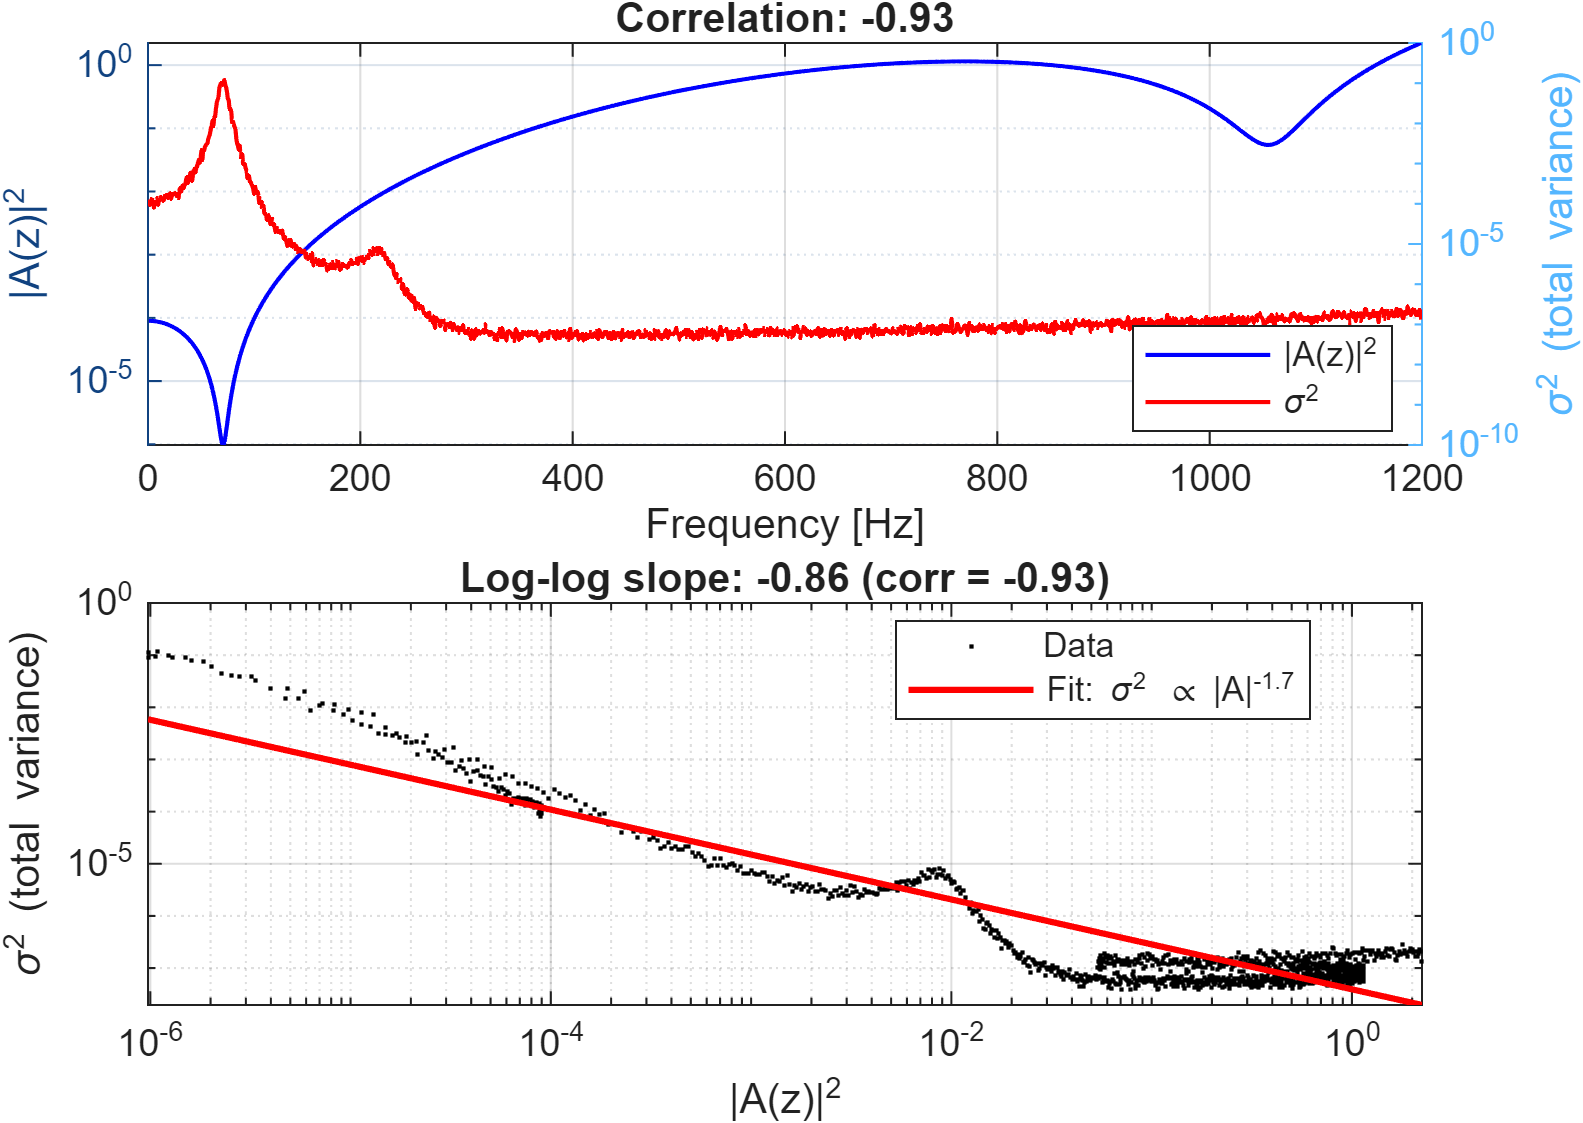
\includegraphics[width=0.9\textwidth]{pic/2_A_vs_Variance_Correlation.png}
    \caption{Correlation between $|A(z)|^2$ and total variance $\sigma_k^2$. Top: both quantities versus frequency showing inverse relationship. Bottom: log-log scatter plot with fitted line($r \approx -0.93$).}
    \label{fig:a_vs_variance}
\end{figure}

IWLS, by contrast, \textbf{removes} this implicit weighting through its $1/|A(z)|^2$ correction. This makes all frequencies contribute equally to the unweighted output error, causing IWLS to overfit the noisy regions near resonances. IWLS achieves the lowest unweighted cost (as designed), but this comes at the expense of the weighted cost.

\textbf{Conclusion:} For systems where stochastic distortion dominates at resonances, LLS can perform surprisingly well. 



\chapter{Model order selection}
\label{chap:model_order}

Selecting appropriate model orders $n_a$ (denominator) and $n_b$ (numerator) is crucial: too few parameters underfit the data, while too many lead to overfitting. We use two complementary criteria.

\section{Corrected Akaike Information Criterion (AICc)}

The AICc balances model fit against complexity:

\begin{equation}
    \text{AICc} = N \ln(V) + 2p + \frac{2p(p+1)}{N-p-1}
\end{equation}

where $N$ is the number of frequency points, $p = n_b + 1 + n_a$ is the number of parameters, and $V$ is the mean squared normalized residual:

\begin{equation}
    V = \frac{1}{N} \sum_{k=1}^{N} \frac{\left| \hat{G}_{\text{ML}}(f_k) - \hat{G}_{\text{model}}(f_k) \right|^2}{\sigma_k^2}
\end{equation}

The correction term $\frac{2p(p+1)}{N-p-1}$ penalizes overparameterization more strongly than standard AIC, making it suitable when $N/p$ is not large.

\section{Whiteness Test}

A correctly specified model should produce residuals that behave like white noise. We test this by computing the normalized autocorrelation of the residuals at lags $\ell = 1, 2, \ldots, L$:

\begin{equation}
    \hat{r}(\ell) = \frac{1}{N} \sum_{k=1}^{N-\ell} \tilde{\varepsilon}_k \tilde{\varepsilon}_{k+\ell}^*
\end{equation}

where $\tilde{\varepsilon}_k = (G_k - \hat{G}_k)/\sigma_k$ is the normalized residual. For white noise, approximately 95\% of the autocorrelation values should fall within $\pm 1.96/\sqrt{N}$. The whiteness percentage indicates model adequacy.

\textbf{Note:} The whiteness test is used only as a \textbf{visual diagnostic} to verify that the selected model adequately captures the system dynamics. The optimal model order is determined \textbf{solely by minimizing AICc}---the whiteness percentage is not incorporated into the selection criterion.

\section{Generalized Information Criterion (GIC)}

The AICc criterion assumes that the residuals are \textbf{white Gaussian noise}. However, this assumption is violated in our case for two reasons:
\begin{enumerate}
    \item \textbf{Stochastic nonlinear distortion:} The Silverbox system exhibits nonlinear behavior. Since we fit a linear model, the residuals contain primarily the stochastic nonlinear distortion, which is not white noise it has frequency-dependent structure.
    \item \textbf{Model mismatch:} The residuals represent the nonlinear contributions that a linear model fundamentally cannot capture, rather than random measurement noise.
\end{enumerate}

When residuals are colored (correlated) rather than white, AICc tends to \textbf{overestimate} the optimal model order, because the effective number of independent observations is lower than $N$.

As an alternative, we also compute the \textbf{Bayesian Information Criterion} (BIC), also known as the Schwarz criterion or Minimum Description Length (MDL):

\begin{equation}
    \text{BIC} = N \ln(V) + p \ln(N)
\end{equation}

\textbf{Comparison of penalties:}
\begin{itemize}
    \item AICc penalty: $2p + \frac{2p(p+1)}{N-p-1} \approx 2p$ for large $N$
    \item BIC penalty: $p \ln(N)$
\end{itemize}

For $N > 8$, we have $\ln(N) > 2$, so BIC penalizes model complexity more strongly than AICc. This makes BIC:
\begin{itemize}
    \item \textbf{More conservative:} Selects lower model orders
    \item \textbf{Consistent:} Asymptotically selects the true model order as $N \to \infty$
    \item \textbf{More robust:} Less sensitive to violations of the white noise assumption
\end{itemize}

For the Silverbox system, where we know the underlying dynamics are 2nd order, BIC often provides a more physically meaningful model order.

\section{Results}

For each parametric estimation method, we compute the AICc, whiteness and BIC across all model orders $(n_a, n_b)$ with $n_a \in \{1, \ldots, 10\}$ and $n_b \in \{0, \ldots, \min(n_a, 10)\}$. The optimal order is selected as the one minimizing AICc (marked with a green circle in the AICc plot, red circle in the whiteness plot).

\subsection{Linear Least Squares (LLS)}

\begin{figure}[H]
    \centering
    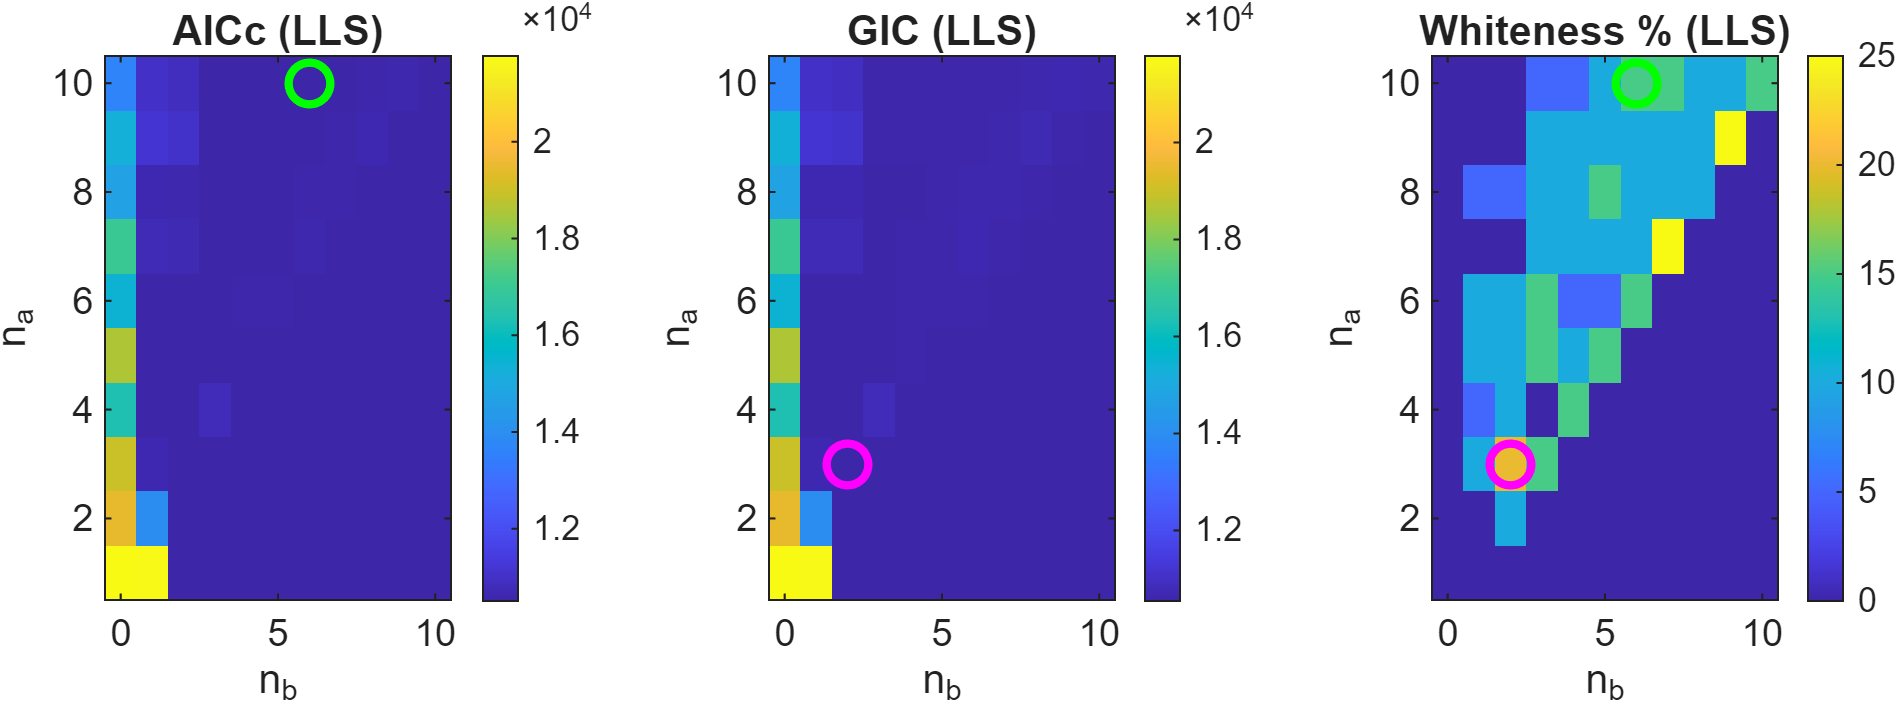
\includegraphics[width=0.9\textwidth]{pic/3_Model_Order_LLS.png}
    \caption{Model order selection using LLS: AICc (left) and whiteness percentage (right). The optimal order is marked with a circle.}
    \label{fig:model_order_lls}
\end{figure}

\subsection{Total Least Squares (TLS)}

\begin{figure}[H]
    \centering
    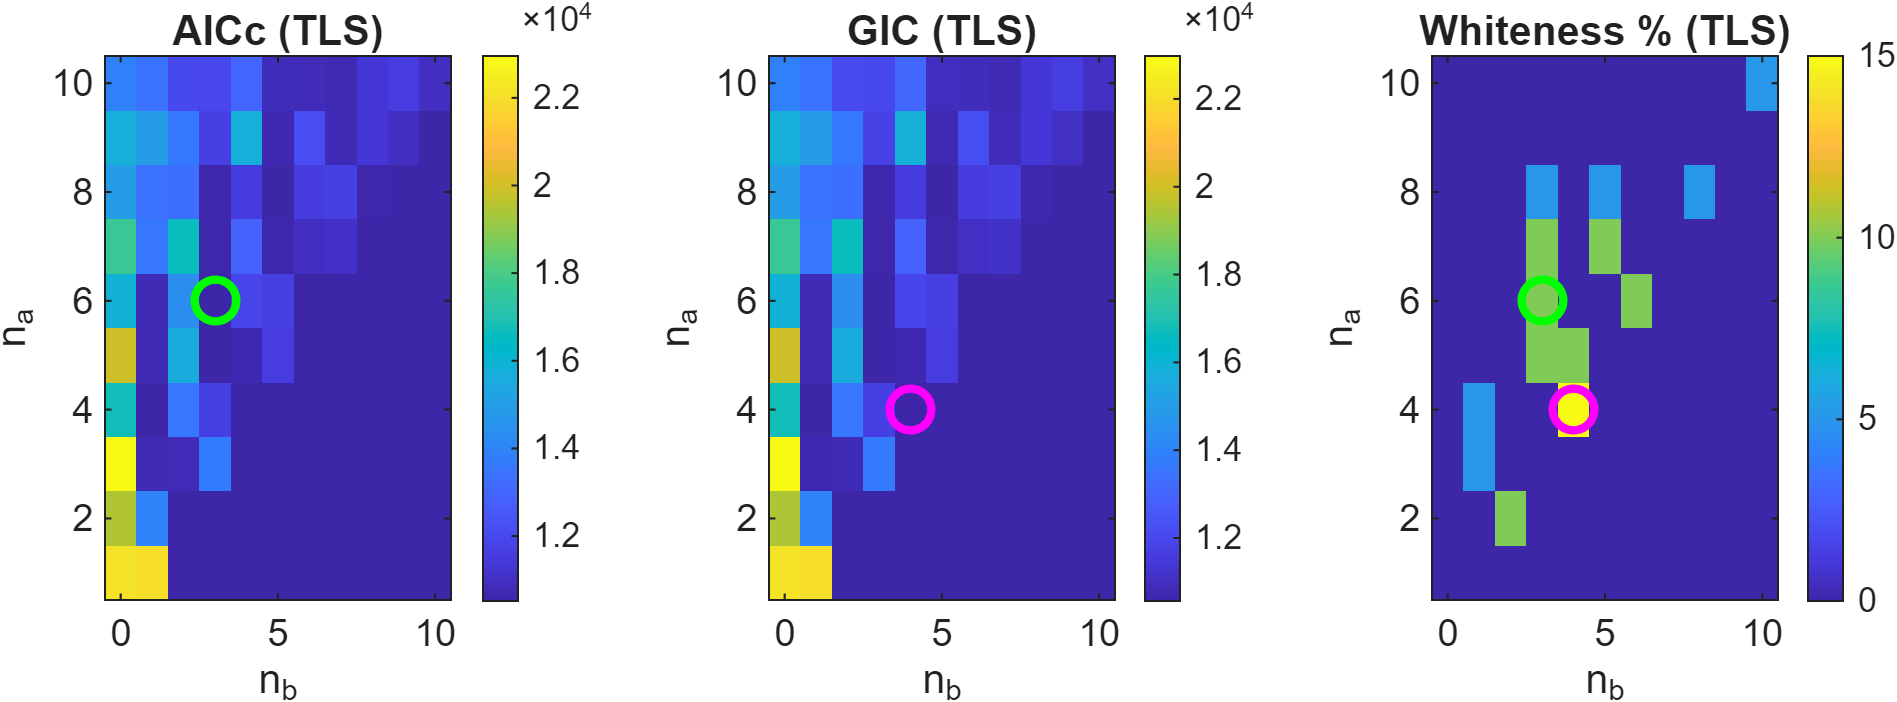
\includegraphics[width=0.9\textwidth]{pic/3_Model_Order_TLS.png}
    \caption{Model order selection using TLS: AICc (left) and whiteness percentage (right). The optimal order is marked with a circle.}
    \label{fig:model_order_tls}
\end{figure}

\subsection{Generalized Total Least Squares (GTLS)}

\begin{figure}[H]
    \centering
    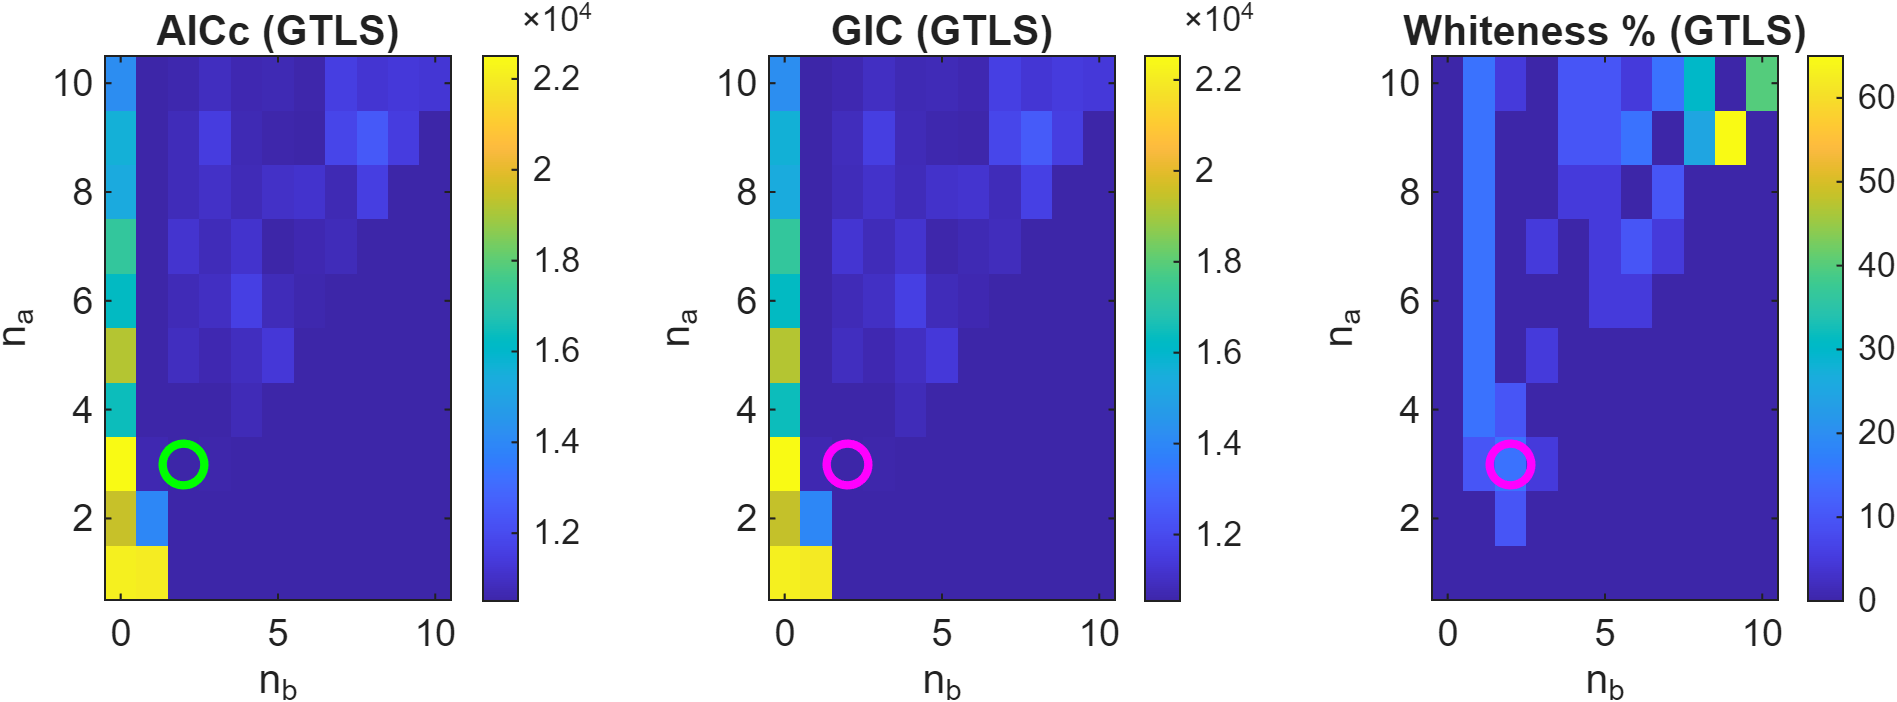
\includegraphics[width=0.9\textwidth]{pic/3_Model_Order_GTLS.png}
    \caption{Model order selection using GTLS: AICc (left) and whiteness percentage (right). The optimal order is marked with a circle.}
    \label{fig:model_order_gtls}
\end{figure}

\subsection{Weighted Least Squares (WLS)}

\begin{figure}[H]
    \centering
    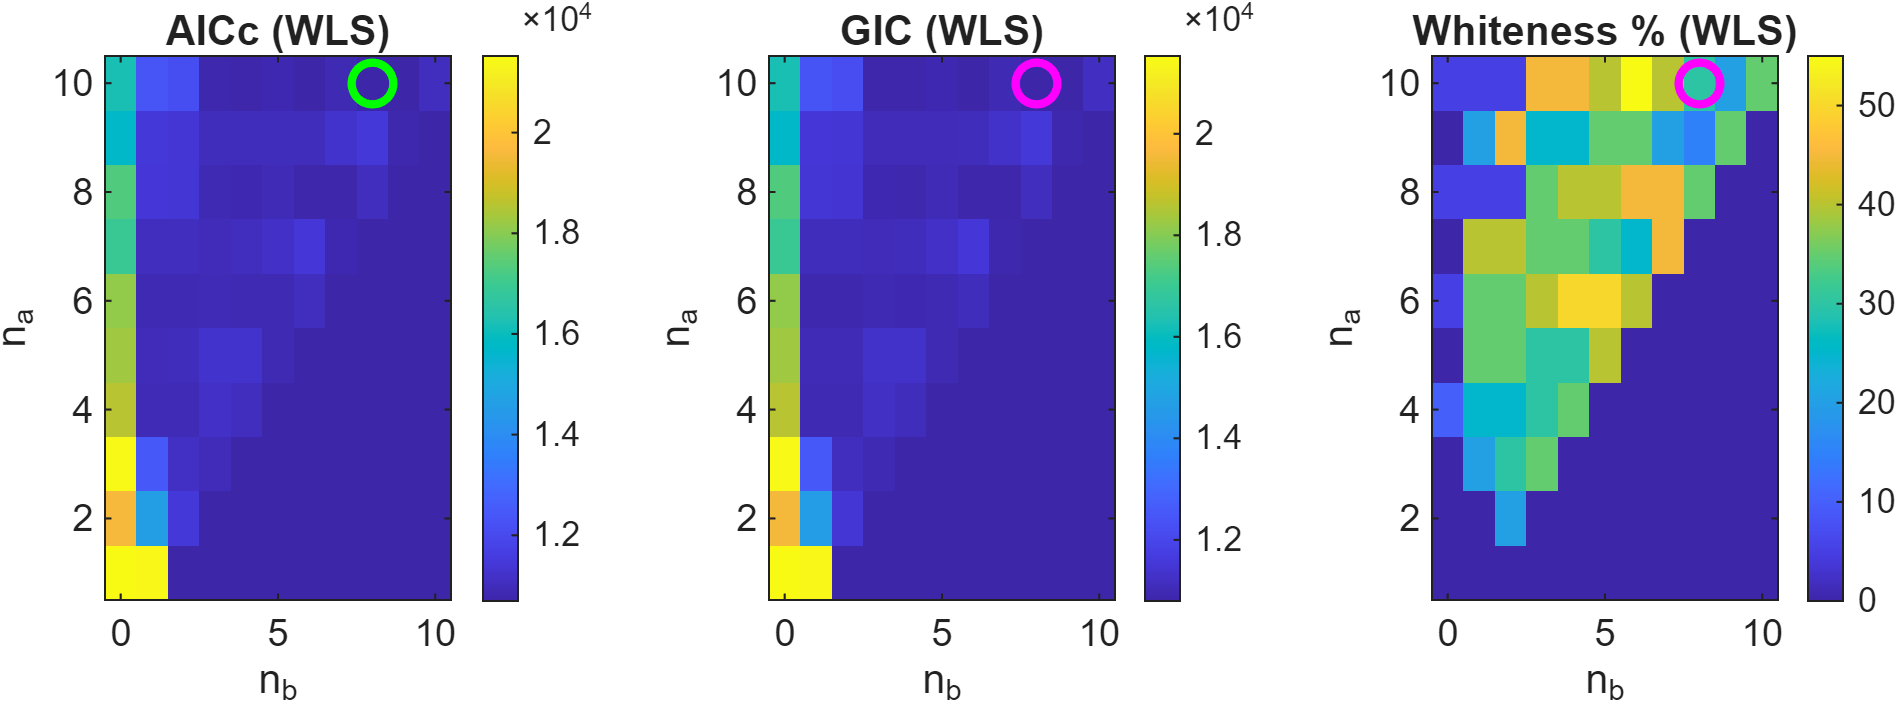
\includegraphics[width=0.9\textwidth]{pic/3_Model_Order_WLS.png}
    \caption{Model order selection using WLS: AICc (left) and whiteness percentage (right). The optimal order is marked with a circle.}
    \label{fig:model_order_wls}
\end{figure}

\subsection{Iterative Weighted Least Squares (IWLS)}

\begin{figure}[H]
    \centering
    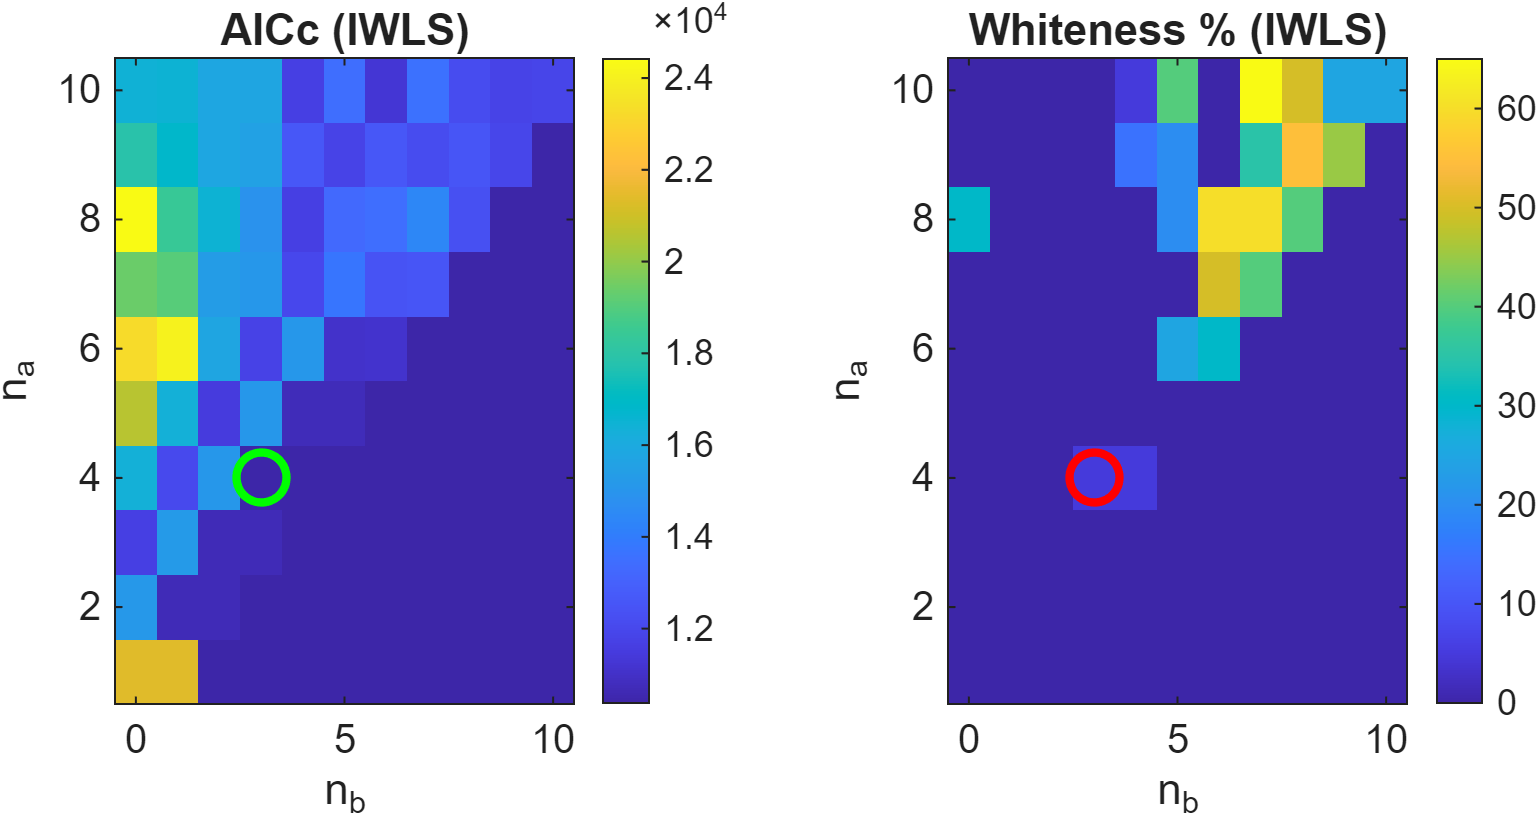
\includegraphics[width=0.9\textwidth]{pic/3_Model_Order_IWLS.png}
    \caption{Model order selection using IWLS: AICc (left) and whiteness percentage (right). The optimal order is marked with a circle.}
    \label{fig:model_order_iwls}
\end{figure}

\subsection{Iterative Quadratic Maximum Likelihood (IQML)}

\begin{figure}[H]
    \centering
    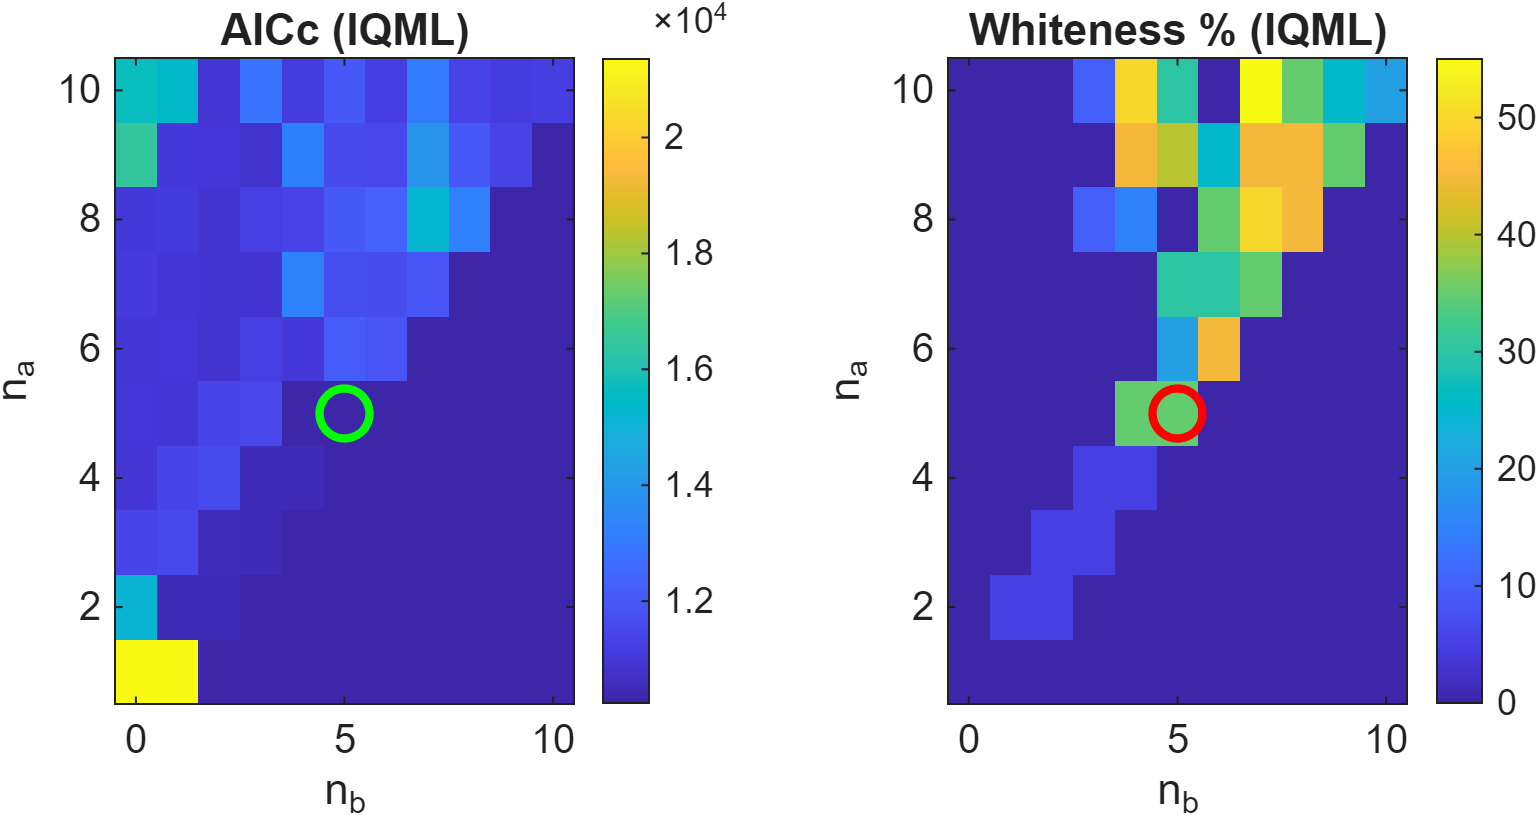
\includegraphics[width=0.9\textwidth]{pic/3_Model_Order_IQML.png}
    \caption{Model order selection using IQML: AICc (left) and whiteness percentage (right). The optimal order is marked with a circle.}
    \label{fig:model_order_iqml}
\end{figure}

\subsection{Maximum Likelihood (ML)}

\begin{figure}[H]
    \centering
    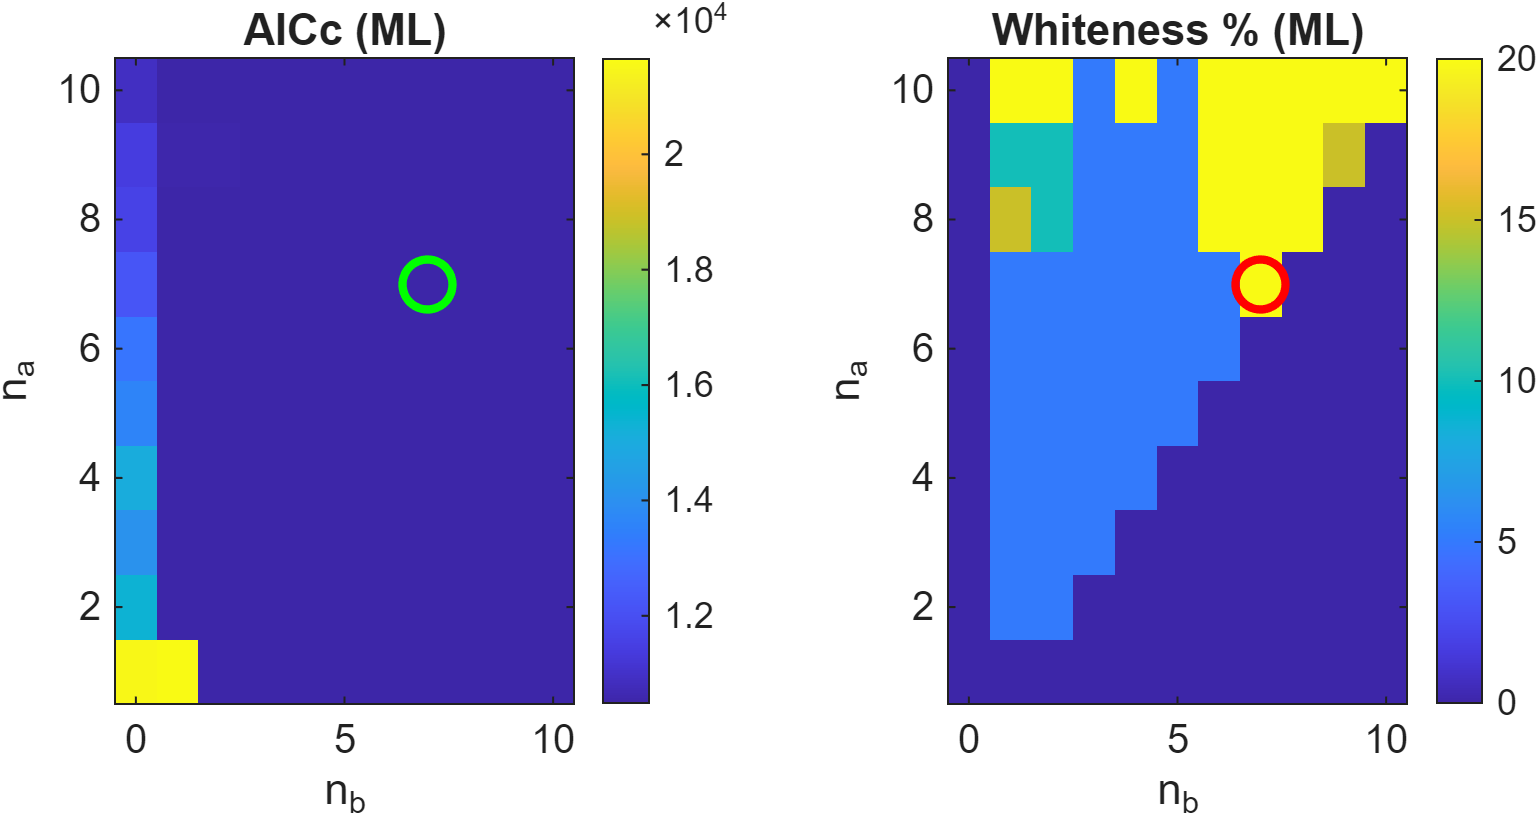
\includegraphics[width=0.9\textwidth]{pic/3_Model_Order_ML.png}
    \caption{Model order selection using ML (Levenberg-Marquardt): AICc (left) and whiteness percentage (right). The optimal order is marked with a circle.}
    \label{fig:model_order_ml}
\end{figure}

\subsection{Comparison Across All Methods}

Table~\ref{tab:model_order_summary} summarizes the optimal model orders selected by each estimation method based on minimum AICc, along with the corresponding whiteness percentage at that order.

\begin{table}[H]
\centering
\begin{tabular}{|l|c|c|c|c|}
\hline
\textbf{Method} & $n_a^*$ & $n_b^*$ & \textbf{AICc} & \textbf{Whiteness (\%)} \\
\hline
LLS & 10 & 6 & 10506.08 & 15.0 \\
\hline
TLS & 6 & 3 & 10516.89 & 10.0 \\
\hline
GTLS & 3 & 2 & 10506.52 & 15.0 \\
\hline
WLS & 10 & 8 & 10695.10 & 30.0 \\
\hline
IWLS & 4 & 3 & 10379.06 & 5.0 \\
\hline
IQML & 5 & 5 & 10243.36 & 35.0 \\
\hline
ML & 7 & 7 & 10488.53 & 20.0 \\
\hline
\end{tabular}
\caption{Optimal model orders $(n_a^*, n_b^*)$ selected by minimizing AICc for each estimation method, with the corresponding whiteness percentage.}
\label{tab:model_order_summary}
\end{table}


Table 4.2 shows the optimal model orders selected by minimizing BIC for each method, along with the corresponding whiteness percentage at that order.


\begin{table}[H]
\centering
\begin{tabular}{|l|c|c|c|c|}
\hline
\textbf{Method} & $n_a^*$ & $n_b^*$ & \textbf{BIC} & \textbf{Whiteness (\%)} \\
\hline
LLS & 3 & 2 & 10545.69 & 20.0 \\
\hline
TLS & 4 & 4 & 10565.67 & 15.0 \\
\hline
GTLS & 3 & 2 & 10538.34 & 15.0 \\
\hline
WLS & 10 & 8 & 10795.53 & 30.0 \\
\hline
\end{tabular}
\caption{Optimal model orders $(n_a^*, n_b^*)$ selected by minimizing BIC for each estimation method.}
\label{tab:model_order_bic}
\end{table}

